\documentclass{article}
\usepackage[top=1.25in, bottom=1.25in, left=1.25in, right=1.25in]{geometry}
\usepackage{amsmath}
\usepackage{natbib}
\usepackage{eufrak}
\usepackage{amsfonts}
\usepackage{mathrsfs}
\usepackage{amsthm}
\usepackage[T1]{fontenc}
\usepackage{tikz-cd}
\usepackage{adjustbox}

\newtheoremstyle{theorem}%    <name>
                {\topsep}%   <space above>
                {\topsep}%   <space below>
                {\normalfont}%  <body font>
                {}%          <indent amount>
                {\bfseries}% <Theorem head font>
                {}%         <punctuation after theorem head>
                {\newline}%  <space after theorem head> (default .5em)
                {}%          <Theorem head spec>
\theoremstyle{theorem}
\newtheorem{theorem}{Theorem}[section]
\newtheorem{corollary}{Corollary}[theorem]
\newtheoremstyle{lemma}%    <name>
                {\topsep}%   <space above>
                {\topsep}%   <space below>
                {\itshape}%  <body font>
                {}%          <indent amount>
                {\bfseries}% <Theorem head font>
                {}%         <punctuation after theorem head>
                {0.5em}%  <space after theorem head> (default .5em)
                {}%          <Theorem head spec>
\theoremstyle{lemma}
\newtheorem{lemma}[theorem]{Lemma}

\newtheoremstyle{definition}%    <name>
                {\topsep}%   <space above>
                {\topsep}%   <space below>
                {\normalfont}%  <body font>
                {}%          <indent amount>
                {\bfseries}% <Theorem head font>
                {.}%         <punctuation after theorem head>
                {\newline}%  <space after theorem head> (default .5em)
                {}%          <Theorem head spec>
\theoremstyle{definition}
\newtheorem{definition}{Definition}[section]
\newtheoremstyle{remark}%    <name>
                {\topsep}%   <space above>
                {\topsep}%   <space below>
                {\normalfont}%  <body font>
                {}%          <indent amount>
                {\bfseries}% <Theorem head font>
                {.}%         <punctuation after theorem head>
                { }%  <space after theorem head> (default .5em)
                {}%          <Theorem head spec>
\theoremstyle{remark}
\newtheorem*{remark}{Remark}

\newcommand\fr[1]{\textcolor{red}{\bf{FR: #1}}}

\begin{document}

\title{Strategic Reasoning about General Game Playing\\ under Imperfect Information\\ \large Technical Report}
\author{Yihui Ilona Zhu and Francesco Belardinelli}
\date{\today}

\maketitle

\section{Preliminaries}
\par In this technical report, we mainly focus on the translation from
Game Description Language with Imperfect Information (GDL-II) to a
Concurrent Game Structure with imperfect information (iCGS) using
Alternating-time Temporal Logic (ATL), as well as the relationship
between the two. This section provides the background information on
the syntax and semantics of GDL-II, and the syntax of ATL and its
semantics over iCGS.


\subsection{GDL-II}

 Game Description Language (GDL) has been well-known for its use
in General Game Playing Competition to define the general rule of a
specific game for a general game player to play. As GDL describes
deterministic actions and states in a game, the type of game that can
be defined by GDL is restricted. Therefore, Game Description Language with Incomplete/Imperfect Information (GDL-II) is developed based on
the general GDL, adding two special keywords, \texttt{sees} and
\texttt{random} \citep{gdlii}:
\begin{itemize}
    \item \texttt{sees} specifies the ability of a specific
      player/agent to receive information of specific ground term (the
      ability to ``perceive" the term);
    \item \texttt{random} represents the occurrence of randomness and chances in some games, which then represent the non-deterministic nature of certain game.
\end{itemize}
This extension allows more games to be represented by GDL-II, such as card games where the players receive random cards and they do not have information about other players' cards. An example of game descriptions in GDL-II is given in Figure 1 on the next page.
\begin{figure}[ht!]
\centering
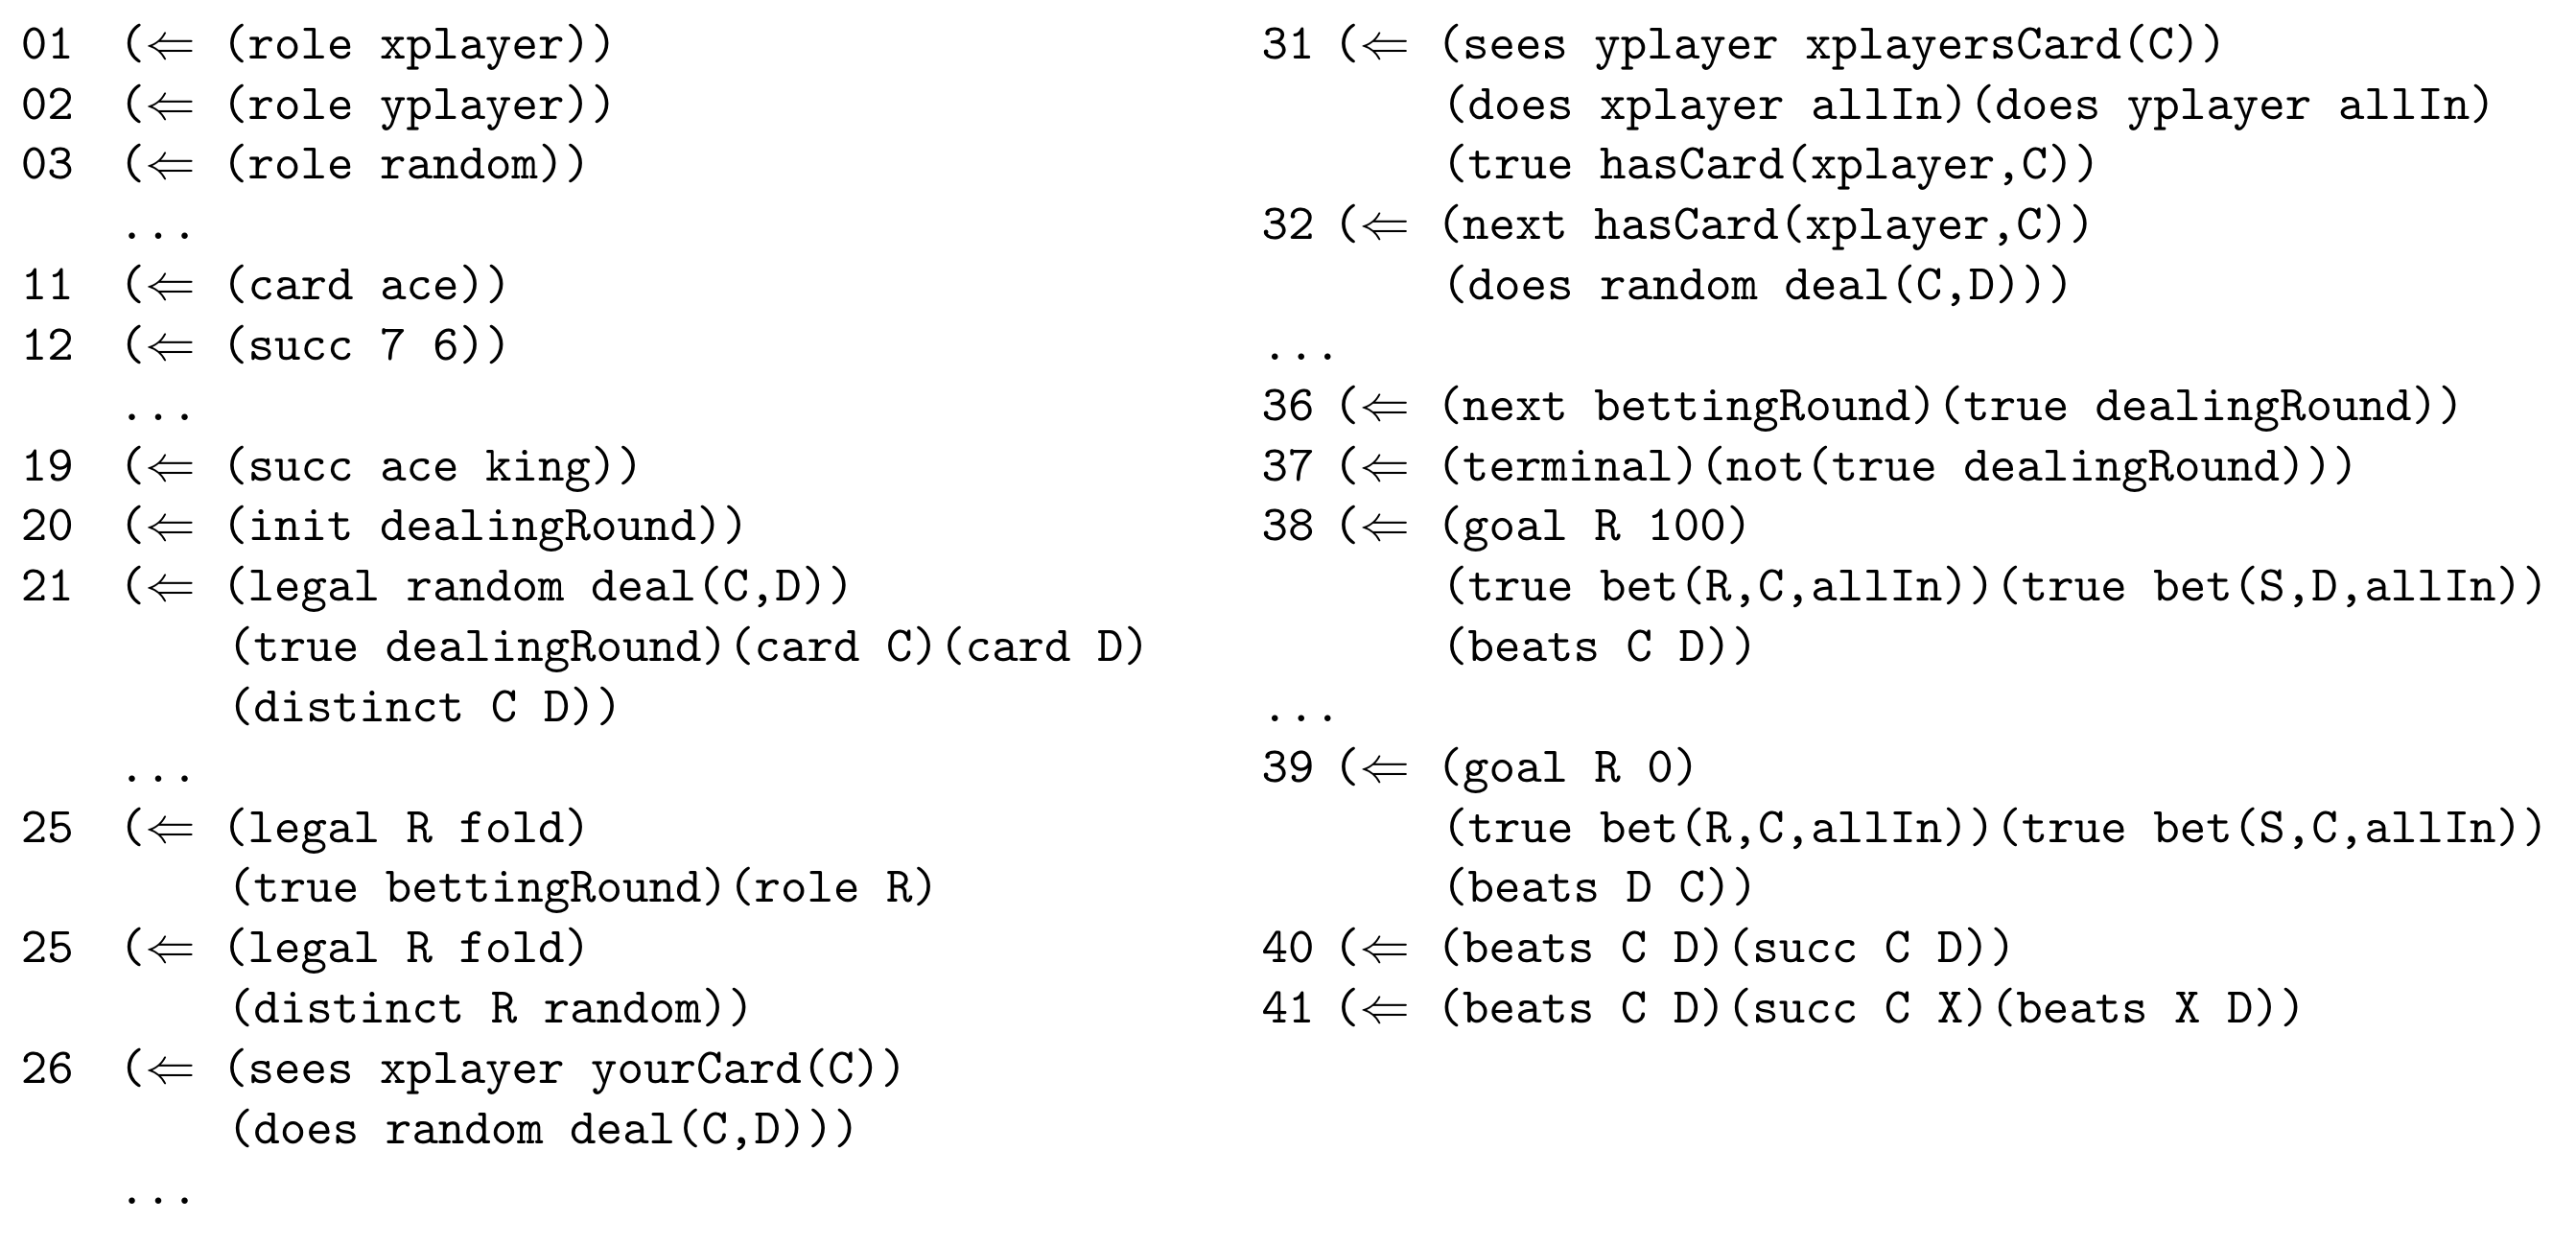
\includegraphics[scale=0.3]{gdl-iiCode.png}
\caption{A fragment of a game description in GDL-II of a simple card game, adapted from \citep{gdlii}.}
\label{fig:gdl-iiCode}
\end{figure}
\par As GDL and GDL-II are based on a logic programming language \textsc{Datalog}, before we can formally define the syntax and
semantics of GDL-II, we begin by acquiring a basic understanding of
\textsc{Datalog}.


\subsubsection{\textsc{Datalog} Program}
\par \textsc{Datalog} is a query and rule language designed for use as a
database language, which syntatically is a subset of \textsc{Prolog}
\citep{datalog}. We now introduce the syntax and semantics for \textsc{Datalog}.
\par This section refers to the same syntax and semantics of \textsc{Datalog}
program presented in \citep{GDLpaper}.
\begin{definition}[\textsc{Datalog} Syntax - Language, Rules and Programs]
    The \textsc{Datalog} Language builds up on a set of atomic propositions $\Pi = \{p,q,\ldots \}$. We denote the set of literals over $\Pi$ by $l(\Pi):l(\Pi)=\Pi \cup \{\neg p\:|\: p \in \Pi \}$.

    A \textsc{Datalog} {\em rule} $r$ is of the form $(\Leftarrow(p)(l_1) \ldots (l_n))$ where $p \in \Pi$ and $l_i \in l(\Pi)(i\leq n)$. The head of $r$ is $p$ in this case: $p=hd(r)$; and the body of $r$, $bd(r)$, is defined as the set $\{l_1,\ldots,l_n \}$, which can be empty in some cases.

    A \textsc{Datalog} {\em program} is a set of \textsc{Datalog} rules.
\end{definition}
 \par In order to understand the semantics of \textsc{Datalog} programs, we
 define a model for \textsc{Datalog} programs as a set of atomic
 propositions which are the atoms that are true. The precise
 definition is below.
\begin{definition}[Models for \textsc{Datalog} Programs]
    Given a \textsc{Datalog} program $\Delta$, a set of atoms $\Sigma \subseteq \Pi$ is a model for $\Delta$ iff it satisfies:
    \begin{itemize}
    \item If $(\Leftarrow(p)) \in \Delta$ then $p \in \Sigma$;
    \item If $(\Leftarrow(p)\,bd) \in \Delta$ and $pos(bd) \subseteq \Sigma$ and $neg(bd) \cap \Sigma=\emptyset$ then $p \in \Sigma$, where $pos(bd)$ is the set of positive literals in $bd$ and $neg(bd)$ is the set of negative ones.
    \end{itemize}
    Following this definition, we can roughly interpret a rule
    $(\Leftarrow (p)(l_1) \ldots (l_n))$ as an implication \allowbreak
    $(l_1 \wedge \ldots \wedge l_n) \rightarrow p$.
\end{definition}
\par In this paper, we focus on stratified \textsc{Datalog} programs, as it is easier to give an interpretation of the semantics of these programs and build their models.
\begin{definition}[Stratified \textsc{Datalog} Programs]
    A \textsc{Datalog} program $\Delta$ is \textit{stratified} if there does not exist circular reasoning in the program. An atom $p$ is in stratum $i \in \mathbb{N}$ if the maximum number of rules $r$ with $p$ as $hd(r)$ and contains the negation of any other atomic proposition in $bd(r)$ is $i$. A rule $r \in \Delta$ is of stratum $i$ if $hd(r)$ is in stratum $i$.
\end{definition}
\begin{definition}[\textsc{Datalog} Semantics for Stratified \textsc{Datalog} Programs]
    Given a stratified \textsc{Datalog} program $\Delta$, we can construct a model for it $s=\textit{DatlogPMod}(\Delta)$. The main idea behind this iterative process is that we first find the heads (atomic propositions) of singleton rules (rules with empty bodies), and then keep going through all the rules and find all the heads of the rules that can be satisfied by the atomic propositions we already have, until nothing can be found.
    
    The procedure is as follows. Firstly, put $t_0=\{p \:|\: (\Leftarrow p) \in \Delta\}$. Now assuming $t_i$ is defined, we initialise $s_i$ to $t_i$, and for all the rules $(\Leftarrow (p)(l_1) \ldots(l_n))$ in stratum $i$ such that $s_i \models l_1 \wedge \ldots \wedge l_n$, add $p$ to $s_i$. Then, let $t_{i+1}=s_i$. Suppose the maximum stratum of $\Delta$ is $k$, then let $s=t_{k+1}$. This $\textit{DatlogPMod}(\Delta)$ is the \textsc{Datalog} semantics of $\Delta$.
\end{definition}

\subsubsection{GDL-II Syntax}
\par We now introduce the formal definition of the syntax of GDL-II game descriptions. This section mainly refers to the GDL syntax discussed in \citep{GDLpaper} with extension to GDL-II rules from \citep{gdlii}.
\begin{definition}[GDL-II Syntax]
    Given a set of agents $Ag$, a special agent \texttt{random}, a set of actions $Ac$, a set of strings $S$, a primitive set of
    propositional atoms $Prim=\{p,q, \ldots \}$, a set of integers $[0 \ldots 100]$ (an arbitrary range) and a set of terms $T$, we define the set of atomic propositions of GDL-II $At_\textsc{gdl-ii}$ as the smallest set that satisfied the following:
    \begin{itemize}
        \setlength\itemsep{0em}
        \item $Prim \subseteq At_\textsc{gdl-ii}$;
        \item special atom \texttt{terminal} $\in At_\textsc{gdl-ii}$;
        \item for all $\texttt{s\textsubscript{1}}, \texttt{s\textsubscript{2}} \in S$, (\texttt{distinct s\textsubscript{1} s\textsubscript{2}}) $\in At_\textsc{gdl-ii}$;
        \item for each agent \texttt{i} $\in Ag \cup \{\texttt{random} \}$ and each action \texttt{a} $\in Ac$, (\texttt{legal i a}) $\in At_\textsc{gdl-ii}$;
        \item for each agent \texttt{i} $\in Ag$, for all integer \texttt{v} in [0,\ldots100], (\texttt{goal i v}) $\in At_\textsc{gdl-ii}$.
    \end{itemize}
    
    We also define $AtExpr_\textsc{gdl-ii}$ - the set of atomic expressions of GDL-II - as the smallest set that satisfies the following:
    \begin{itemize}
        \setlength\itemsep{0em}
        \item for each \texttt{p} $\in At_\textsc{gdl-ii}$, \{(\texttt{p}), (\texttt{init p}), (\texttt{next p}), (\texttt{true p})\} $\subseteq AtExpr_\textsc{gdl-ii}$;
        \item for each agent \texttt{i} $\in Ag \cup \{\texttt{random} \}$ and each action \texttt{a}, \{(\texttt{role i}), (\texttt{does i a})\} $\subseteq AtExpr_\textsc{gdl-ii}$;
        \item for each agent \texttt{i} $\in Ag$ and each term \texttt{t} $\in T$, (\texttt{sees i t}) $\in AtExpr_\textsc{gdl-ii}$.
    \end{itemize}
    
    $LitAt_\textsc{gdl-ii}$ is defined as $\{\texttt{p}, (\texttt{true p}), (\texttt{not p}), (\texttt{not}\,(\texttt{true p}))\:|\: \texttt{p} \in At_\textsc{gdl-ii}\}$. Finally, we define $LitExpr_\textsc{gdl-ii}$ as $AtExpr_\textsc{gdl-ii} \cup LitAt_\textsc{gdl-ii}$.
\end{definition}
\par We also enforce some restrictions on the use of the keywords in GDL-II:
\begin{itemize}
    \item \texttt{role} only appears in the head of rules;
    \item \texttt{init} only appears as head of rules and does not depend on any of the other keywords;
    \item \texttt{true} only appears in the body of rules;
    \item \texttt{does} only appears in the body of rules and does not depend on \texttt{legal}, \texttt{terminal} or \texttt{goal};
    \item \texttt{next} and \texttt{sees} only appear as head of rules.
\end{itemize}
\par Now, because \texttt{true p} and \texttt{p} have the same meaning, the keyword \texttt{true} does not really extend the expressive power of GDL or GDL-II. Hence, in this report, we omit \texttt{true} from the rules and proofs of results for GDL-II, i.e.\ in the following sections of this report, we only include \texttt{p} and the corresponding proofs for \texttt{true p} are the same.
\par A \textit{game description} specifies all the atoms from $At_\textsc{gdl-ii}$ that are true, in one of the following situations: true in the initial state, true as a result of global constraints, or true as the effect of some joint actions being performed in a specific state. The semantics of atomic expressions will be given using the definition below and game model constructed later.
\begin{definition}[Game Descriptions]
    A GDL-II game description $\Gamma$ is a set of \textsc{Datalog} rules $r$ of the form ($\Leftarrow$(\texttt{h})(\texttt{e\textsubscript{1}})\ldots (\texttt{e\textsubscript{m}})), where the head of the rule $\texttt{h}=hd(r)$ is from $AtExpr_\textsc{gdl-ii}$ and each \texttt{e\textsubscript{i}}($i\in[1\ldots m]$) in $bd(r)$ is from $LitExpr_\textsc{gdl-ii}$. We say $r$ has an \textit{empty body} if $m=0$. For our convenience, we categorise every game description $\Gamma$ into five different types of rules where:
    \begin{itemize}
        \item $\Gamma_\texttt{init}$ contains all the rules that represent constraints of the initial state of the game, i.e.\ rules of the form ($\Leftarrow (\texttt{init p})$). These rules have a head only and an empty body;
        \item $\Gamma_\texttt{role}$ contains all the rules that specify the agents of the game, i.e.\ rules of the form \\ $(\Leftarrow(\texttt{role i}))$;
        \item $\Gamma_\texttt{glob}$ contains all the global constraints, which are the rules of the form $(\Leftarrow(\texttt{p}) (\texttt{e\textsubscript{1}}) \ldots(\texttt{e\textsubscript{m}}))$, where \texttt{p} $\in At_\textsc{gdl-ii}$ and each $\texttt{e\textsubscript{i}}$($i \in [1\ldots m]$) is from  $LitAt_\textsc{gdl-ii}$;
        \item $\Gamma_\texttt{next}$ contains all rules with a (\texttt{next p}) in the head: $(\Leftarrow(\texttt{next p}) (\texttt{e\textsubscript{1}}) \ldots (\texttt{e\textsubscript{m}}))$, where \texttt{p} $\in At_\textsc{gdl-ii}$ and each $\texttt{e\textsubscript{i}}$($i \in [1\ldots m]$) is from  $LitAt_\textsc{gdl-ii}$ or of the form (\texttt{does i a});
        \item $\Gamma_\texttt{sees}$ contains all rules with a (\texttt{sees i t}) in the head: $(\Leftarrow(\texttt{sees i t}) (\texttt{e\textsubscript{1}}) \ldots(\texttt{e\textsubscript{m}}))$, where each $\texttt{e\textsubscript{i}}$ ($i \in [1\ldots m]$) is from $LitAt_\textsc{gdl-ii}$ or of the form (\texttt{does i a}).
    \end{itemize}
\end{definition}
\par We also assume that any given game description $\Gamma$ will be stratified according to Def.~1.3.


\subsubsection{GDL-II Semantics: Game Model}

Although the developer of GDL-II already provided a game model for
GDL-II in \citep{gdlii}, that game model is not clear
enough. Furthermore, as the agent does not have perfect information
about the game, situations where an agent cannot distinguish between
two states might occur, and the game model should be able to describe
these situations. Therefore, for the description of a different game
model $G$, we use the same approach as in \citep{GDLpaper} but
with some slight changes. Again, this section refers to the game model
constructed for GDL in \citep{GDLpaper} with modifications to extend
it to GDL-II.
\begin{definition}[GDL-II Game Model]
    Given the set of atomic propositions $At_\textsc{gdl-ii}$, a GDL-II Game Model is a tuple
%    \begin{center}
        $G  =  \langle S, s_{0}, Ag, \{Ac_{i}\}_{i \in Ag}, \allowbreak \{ \sim_i \}_{i \in Ag}, \tau, \pi \rangle$
%    \end{center}
    where
    \begin{itemize}
        \item $S$ is a finite non-empty set of states, with $s_{0}$ the initial state;
      \item $Ag$ is the a finite non-empty set of agents in the game, including the \texttt{random} agent;
      \item each $Ac_{i}$ is a finite non-empty set of possible actions for a specific agent $i$;
       \item each indistinguishability relations $\sim_i$ specify the situations where an agent $i$ cannot distinguish between two states in a game.
      \item $\tau: Ac_{1}\times  \ldots \times Ac_{n} \times S \rightarrow S$ is an update function that takes a state and one action taken by each agent, and then returns the successor state;
      \item $\pi:S \rightarrow 2\textsuperscript{\textit{At}\textsubscript{\textsc{gdl}}}$ is an interpretation function that takes a state and returns a set of atomic propositions that are satisfied in the state.
    \end{itemize}
\end{definition}

\par For our game models, they are pretty much the same as those of \citep{GDLpaper}. However, as the game descriptions now involve imperfect information, we define certain components differently in order to incorporate the \texttt{sees} expressions.
\par Now we construct all the components of the game model $G$ for a game description $\Gamma$. The set of agents $Ag$ follows from the game description $\Gamma$: $Ag = \{i\:|\: (\Leftarrow (\texttt{role i})) \in \Gamma_\texttt{role} \} \cup \{\texttt{random}\}$. The set of actions for each agent $i$ - $Ac_i$ - also follows from $\Gamma$: $Ac_i = \{\texttt{a}\:|\: (\texttt{legal i a}) \text{ occurs in } \Gamma \}$. The main idea behind constructing all the states in the game is that we think of every state $s \in S$ as associated with the unique model under the semantics of some stratified \textsc{Datalog} program $\Delta$ derived from $\Gamma$. Particularly, we let $\delta(\Gamma_\texttt{glob})$ and $\delta(\Gamma_\texttt{init})$ be derived from $\Gamma$, where $\delta(\Gamma_\texttt{glob})$ is the set of global rules where we treat all the \texttt{true p} atoms as \texttt{p} atoms and $\delta(\Gamma_\texttt{init})$ is the set \{$\Leftarrow \texttt{p}
\:|\: (\texttt{init p}) \in \delta(\Gamma_\texttt{init})$\}.  \par The steps below outline the procedure of constructing $S$, $\tau$, and $\pi$ used in $G$.
\begin{itemize}
    \item \textit{Firstly}, we define the initial state $s_0$. Put
    \begin{center}
        $\pi(s_{0}) = \textit{DatlogPMod}(\delta(\Gamma_\texttt{init}) \cup \delta(\Gamma_\texttt{glob}))$
    \end{center}
    Since $\delta(\Gamma_\texttt{glob})$ is stratified whenever
    $\Gamma_\texttt{glob}$ is, we obtain that the given game
    description $\Gamma$ is stratified, and we ensure we are applying
    $\textit{DatlogPMod}$ to a stratified program. Additionally,
    \texttt{sees} atoms only appear as the head of a rule, and the
    body only consists of global constraints and \texttt{does}
    expressions. We can therefore deduce that no \texttt{sees} atoms
    will appear in the initial state as no actions have been taken at
    this point, so we only consider $\delta(\Gamma_\texttt{init})$ and
    $\delta(\Gamma_\texttt{glob})$ here.
    \item \textit{Next}, we generate the finite non-empty set of
      states $S$. We begin by supposing that a state $s \in S$ has
      been defined already. This is in fact true as we begin this step
      after having defined the initial state $s_0$, so that we would
      always have some states already defined in $S$. We also know
      from the way the game description is developed that if this
      state $s$ is not a terminal state ($\texttt{terminal} \notin
      \pi(s)$), every agent has at least one legal action available in
      the state. The way we classify these legal actions is by
      checking that for action $a_i$ $(\texttt{legal i
        a\textsubscript{i}}) \in \pi(s)$. If we know that
      $\texttt{terminal} \notin \pi(s)$, there exists a successor
      state $u$ of $s$ after a profile of legal actions $\langle{a_1,
        \ldots, a_n}\rangle$ is performed, i.e., each agent performs
      one legal action out of all available legal actions for that
      agent. For each possible profile of legal actions $\langle{a_1,
        \ldots, a_n}\rangle$, we define $u$ by first computing all
      atoms that should be satisfied (true) in the next state according to $\Gamma_\texttt{next}$, using a modified version of the function
      $F_\Gamma$ from \citep{GDLpaper} that considers the
      \texttt{sees} atoms arising from imperfect information.
      \begin{eqnarray*}
      F_\Gamma(\langle{a_1, \ldots, a_n}\rangle, s) & = & \{\Leftarrow
      \texttt{p}\:|\: \text{there exists some }
      (\Leftarrow(\texttt{next
        p})(\texttt{e\textsubscript{1}})\ldots(\texttt{e\textsubscript{k}}))
      \in \Gamma_\texttt{next} \text{ and}\\ & & \pi(s) \cup \{ \neg
      q\,|\,q\notin \pi(s) \} \cup \{(\texttt{does i
        a\textsubscript{i}})\,|\,i \in [1\ldots n]
      \}\models_\textit{cl} \texttt{e\textsubscript{1}} \wedge \ldots
      \wedge \texttt{e\textsubscript{k}} \}\\ & & \cup \,\{ \Leftarrow
      (\texttt{sees i t})\:|\: \text{there exists some }\\ & &
      (\Leftarrow(\texttt{sees i t})
      (\texttt{e\textsubscript{1}})\ldots(\texttt{e\textsubscript{k}}))
      \in \Gamma_\texttt{sees} \text{ and}\\ & & \pi(s) \cup \{ \neg
      q\,|\,q\notin \pi(s) \} \cup \{(\texttt{does i
        a\textsubscript{i}})\,|\,i \in [1\ldots n]
      \}\models_\textit{cl} \texttt{e\textsubscript{1}} \wedge \ldots
      \wedge \texttt{e\textsubscript{k}} \}
    \end{eqnarray*}
    Now that we have a set of atoms that need to be satisfied in the next state (when each agent $i$ takes an action $a_i$), we can add a new state to the game model and put
    \begin{center}
        \par $u = \tau(\langle{a_1, \ldots, a_n}\rangle, s)$ \par and
        $\pi(u) = \textit{DatlogPMod}(F_\Gamma(\langle{a_1, \ldots,
          a_n}\rangle, s)\cup \delta(\Gamma_\texttt{glob}))$
    \end{center}
    \item \textit{Iteration:} repeat the step above to all successor
      states of the initial state, until reaching all terminal states
      of the game.
\end{itemize}
\par Now, we can define the indistinguishability relation $\sim_{i}$,
which describes an agent $i$ cannot distinguish between two states $q$
and $q'$, and is defined as $q \sim_{i} q'$ iff for all terms
\textit{t}:
\begin{itemize}
    \item ($\texttt{sees i t}) \in q \text{ iff } (\texttt{sees i t}) \in q'$, meaning that the agent $i$ receives the exact same information in states $q$ and $q'$;
    \item if ($\texttt{sees i t})\text{ is true then } val(\texttt{t}, q) = val(\texttt{t}, q')$, where $val(t,q)$ returns the valuation of term $\texttt{t}$ in state $q$. This means that $\texttt{t}$ needs to be of the same value in both states if the agent $i$ receives information about the term;
    \item ($\texttt{legal a i}) \in \pi(q) \text{ iff } (\texttt{legal a i}) \in \pi(q')$, meaning that the available actions for agent $i$ are the same in states $q$ and $q'$, ensuring that all strategies are uniform.
\end{itemize}
\begin{lemma}
The indistinguishability relation defined above is an equivalence relation.
\end{lemma}
\begin{proof}
  We will prove the lemma by showing the indistinguishability relation $\sim_i$ is reflexive, symmetric and transitive. Suppose we have an arbitrary agent $i \in Ag$.

  Firstly, suppose we have an arbitrary state $q$. It is then very trivial to see that if we have ($\texttt{sees i t}) \in q$, then $(\texttt{sees i t}) \in q$ is true too, and vice versa. Also, it is very obvious that whenever (\texttt{sees i t}) is true then $val(t, q) = val(t, q)$. Similarly, ($\texttt{legal a i}) \in \pi(q) \text{ iff } (\texttt{legal a i}) \in \pi(q)$ holds. Therefore, we have for all $q \in S, q \sim_i q$, showing that $\sim_i$ is reflexive.

  Secondly, suppose we have two arbitrary states $q$ and $q'$ and assume we have $q \sim_i q'$. We need to show that $q' \sim_i q$. From the assumption, we have ($\texttt{sees i t}) \in q \text{ iff } (\texttt{sees i t}) \in q'$, if ($\texttt{sees i t})\text{ is true then } val(t, q) = val(t, q')$ and ($\texttt{legal a i}) \in \pi(q) \text{ iff } (\texttt{legal a i}) \in \pi(q')$. It is then easy to see that ($\texttt{sees i t}) \in q' \text{ iff } (\texttt{sees i t}) \in q$, ($\texttt{legal a i}) \in \pi(q') \text{ iff } (\texttt{legal a i}) \in \pi(q)$, and if ($\texttt{sees i t})\text{ is true then } val(t, q') = val(t, q)$ all follow directly from our assumption, by the symmetric property of `iff' ($\leftrightarrow$) and the symmetric property of `$=$'. We can now deduce that for all $q, q' \in S,$ if $q \sim_i q'$ then $q' \sim_i q$, so $\sim_i$ is symmetric.
\par Finally, suppose we have three arbitrary states $q$, $q'$ and $q''$, and assume we have $q \sim_i q'$ and $q' \sim_i q''$. We need to show that $q \sim_i q''$. For the first condition, we have ($\texttt{sees i t}) \in q \text{ iff }\\ (\texttt{sees i t}) \in q'$ and ($\texttt{sees i t}) \in q' \text{ iff } (\texttt{sees i t}) \in q''$ from our assumption. Therefore, by transitivity of `iff' ($\leftrightarrow$), we have ($\texttt{sees i t}) \in q \text{ iff } (\texttt{sees i t}) \in q''$. Similarly, the second condition follows directly from the assumption by transitivity of equals (`$=$'), so we have if ($\texttt{sees i t})\text{ is true }\\ \text{then } val(t, q) = val(t, q'')$. The last condition works exactly as the first one - ($\texttt{legal a i}) \in \pi(q) \text{ iff } (\texttt{legal a i}) \in \pi(q'')$ follow from transitivity of `iff' ($\leftrightarrow$). We can then conclude that $\sim_i$ is transitive by for all $q, q', q'' \in S,$ if we have $q \sim_i q$ and $q' \sim_i q''$, then $q \sim_i q''$.
\end{proof}
\par After we construct the model $G$, we can easily verify that it is indeed a game model for $\Gamma$ with the following definitions.
\begin{definition}[GDL-II Semantics]
    Given that we have constructed a game model $G=\langle{S, s_{0}, Ag, Ac_{1}, .., Ac_{n}, \{ \sim_i \}_{i \in Ag}, \tau, \pi}\rangle$ with a family of indistinguishability relations, let $Ag' = \{i_1,\ldots,i_k \}$ be a set of agents $\subseteq Ag$, each agent with an action $a_x$($x \leq k$). Then, we define \textit{t} to be an $i_1: a_1,\ldots,i_k:a_k$ successor of \textit{s} if there exists a choice for any agent $j\in$ \textit{Ag}\textbackslash \textit{Ag'} for an action $b_j$ from $Ac_j$ such that $\tau(\langle{c_1,\ldots,c_n}\rangle)=t$, where $c_y=a_x$ if $y=i_x \in Ag$ and $c_y=b_j$ if $y=j \in$ \textit{Ag}\textbackslash \textit{Ag'}. Given a game model $G$, a state $s$, and $\texttt{p} \in At_\textsc{gdl-ii}$, we define:
    \begin{tabbing}
    \hspace{0.5cm} \= \hspace*{8cm}\= \kill
    \> $G,s \models_\textsc{gdl-ii} \texttt{p}$ \> iff $\texttt{p} \in \pi(s)$;\\
    \> $G,s \models_\textsc{gdl-ii} \texttt{not p}$ \> iff $G,s \not \models_\textsc{gdl-ii} \texttt{p}$;\\
    \> $G \models_\textsc{gdl-ii} (\Leftarrow (\texttt{init p}))$ \> iff $G,s_0 \models_\textsc{gdl-ii} \texttt{p}$;\\    
    \> $G \models_\textsc{gdl-ii} (\Leftarrow(\texttt{p}) (\texttt{e\textsubscript{1}}) \ldots(\texttt{e\textsubscript{m}}))$\\
    \>\hspace{1cm} iff for all $s:($if for each $i \in [1\ldots m].\ G, s \models_\textsc{gdl-ii} \texttt{e\textsubscript{i}}\text{, then } G,s \models_\textsc{gdl-ii} \texttt{p}$);\\
    \> $G \models_\textsc{gdl-ii} (\Leftarrow(\texttt{next p}) (\texttt{e\textsubscript{1}}) \ldots(\texttt{e\textsubscript{m}}) (\texttt{does i\textsubscript{1} a\textsubscript{1}}) \ldots(\texttt{does i\textsubscript{k} a\textsubscript{k}}))$ \\
    \>\hspace{1cm} iff for all $s,t:((\text{if for each } i \in [1\ldots m].\ G, s \models_\textsc{gdl-ii} \texttt{e\textsubscript{i}}\text{ and }$ \\
    \>\hspace{3.4cm} $t \text{ is an } i_1:a_1,\ldots,i_k:a_k \text{ successor of }s)\text{, then } G,t \models_\textsc{gdl-ii} \texttt{p}$);\\
    \> $G \models_\textsc{gdl-ii} (\Leftarrow(\texttt{sees x t}) (\texttt{e\textsubscript{1}}) \ldots(\texttt{e\textsubscript{m}}) (\texttt{does i\textsubscript{1} a\textsubscript{1}}) \ldots(\texttt{does i\textsubscript{k} a\textsubscript{k}}))$\\
    \>\hspace{1cm} iff for all $s,t:((\text{if for each } i \in [1\ldots m].\ G, s \models_\textsc{gdl-ii} \texttt{e\textsubscript{i}}\text{ and }$\\
    \>\hspace{3.4cm} $t \text{ is an } i_1:a_1,\ldots,i_k:a_k \text{ successor of }s)\text{, then } G,t \models_\textsc{gdl-ii} (\texttt{sees x t}$)).
    \end{tabbing}
    With this definition, we ensure that the constructed game model $G \models_\textsc{gdl-ii} \Gamma$.
\end{definition}


\subsection{ATL}
\par Alternating-time Temporal Logic, also known as ATL, is a branching-time logic that extends CTL to multiple agents, where it describes many possible paths for the future, one of which will be the actual path \citep{ctl}. The key element of ATL is the \textit{cooperation modalities} $\langle{\langle{A}\rangle}\rangle$, where $A \subseteq \mathbb{A}\mathrm{gt}$ is a set of agents. Another key formula of ATL is $\langle{\langle{A}\rangle}\rangle \gamma$, where $\gamma$ is a temporal formula. This formula expresses that the coalition (set of agents) $A$ has a \textit{collective strategy} such that $\gamma$ is true. A temporal formula is built using unary operators - $\bigcirc$ meaning `in the next state', $\square$ meaning `always', $\Diamond$ meaning `eventually' - and a binary operator $\mathcal{U}$ meaning `until' \citep{GDLpaper}. In this paper, we focus on the language of ATL only, meaning that each temporal operator must be directly following a cooperation modality.
\begin{definition}[Language $\mathscr{L}_\textsc{atl}$ \citep{cgs}]
    Let $Ag$ be a set of agents and $\Phi$ be a set of atomic propositions, the language $\mathscr{L}_\textsc{atl}$ is given by all formulae generated by the following grammar:
    \begin{center}
        \par $\varphi ::= p\:|\: \neg \varphi \:|\: \varphi \vee \varphi \:|\: \langle{\langle{A}\rangle}\rangle \bigcirc \varphi \:|\: \langle{\langle{A}\rangle}\rangle \square \varphi \:|\: \langle{\langle{A}\rangle}\rangle \varphi \: \mathcal{U} \varphi$
    \end{center}
    where $p \in \Phi$ is a atomic proposition and $A \subseteq Ag$ is a set of agents.
\end{definition}


\subsubsection{ATL Semantics: iCGS}
\par In this paper, the semantics of ATL Language $\mathscr{L}_\textsc{atl}$ is defined over a variant of transition systems - \textit{imperfect information concurrent game structure} (iCGS), which links each transition with a set of actions performed, one by each agent. This section refers to iCGS presented in \citep{cgs} and the ATL semantics refers to the ATL semantics in \citep{GDLpaper} adapted to the definition of \textit{strategies} in \citep{cgs}.
\begin{definition}[iCGS]
    An iCGS is a tuple
%    \begin{center}
        $\mathfrak{M} = \langle{Ag, St, \Pi, \pi, Act, d, o, \{\sim_{i}\}_{i \in Ag}} \rangle$
%    \end{center}
    where
    \begin{itemize}
        \item $Ag$ is a finite non-empty set of all agents involved in the system;
        \item $St$ is a finite non-empty set of states;
        \item $\Pi$ is a finite non-empty set of atomic propositions;
        \item $\pi$ is a valuation function $\pi : \Pi \rightarrow \mathscr{P}(St)$ that returns a set of states in which a specific atomic proposition is satisfied;
        \item $Act$ is a finite non-empty set of actions;
        \item $d : Ag \times St \rightarrow \mathscr{P}(Act)$ is a function  that returns a finite non-empty set of available actions for a specific agent in a specific state. We also use $d_a(q)$ for short for $d(a,q)$;
        \item $o$ is the state transition function that defines the outcome state ($q' = o(q, a_{1}, \ldots, a_{k})$) to a state when a joint move (one action per agent) is carried out;
        \item each indistinguishability relations $\sim_{i} \subseteq St \times St$ represent the uncertainty for the specific agent: $q_{1} \sim_{i}  q_{2}$ means that agent $i$ cannot distinguish between state $q_{1}$ and state $q_{2}$.
    \end{itemize}
\end{definition}
\par The indistinguishability relations are very important as it restricts the semantics of the system - the agent should have the exact same choices in two states that are indistinguishable, which would result in a certain strategy returning the same outcome as the agent has the same information and is bound to play the same action.
\begin{remark}
A concurrent game structure (CGS) under perfect information can be thought of as an iCGS where the indistinguishability relation for each agent is the identity relations that takes two states and returns true only when the two input states are identical.
\end{remark}
\par When it comes to describe the strategy for agents in iCGS, an \textit{imperfect information strategy}, or \textit{uniform strategy}, of an agent is a sequence of actions but with the agent's epistemic limitations \citep{cgs}. This means that the choices for the agent in indistinguishable states must be the same, in order for a strategy to be executable. For our iCGS, we assume all the choices that the agents make are based on the current state only (not including \textit{histories} - previous states). Therefore, we restrict the possible strategies by the following:
\begin{itemize}
    \item An \textit{imperfect information memoryless strategy} ($ir$-strategy) for an agent $i$ is an uniform $Ir$-strategy, which is given by a function $s_i:St \rightarrow Act$, where $s_i(q) \in d_i(q)$, and satisfies the following constraints: if $q \sim_i q'$ then $s_i(q)=s_i(q')$.
    \item A \textit{collective ir-strategy} is a combination of individual $ir$-strategies. $\sum_{i}^{ir}$ denotes the set of the agent $i$'s $ir$-strategies. The set of $A$'s collective imperfect information memoryless strategies is denoted by $\sum_{A}^{ir}=\prod_{i \in A}^{} \sum_{i}^{ir}$. $\sum_{}^{ir} = \sum_{Ag}^{ir}$ gives the set of all strategy profiles of the system.
\end{itemize}
\par Function $out(q,s_A)$ returns the set of all future paths that may occur as a result of the agents $A$ execute strategy $s_A$ from the state $q$ and onward. This set is given by:
\begin{eqnarray*}
    out(q,s_A) & = & \{\lambda=q_0 q_1 q_2\ldots \:|\: q_0=q \text{ and for all } i=1,2,\ldots\text{ there exists a tuple of agents'}\\
    & & \text{decisions } \langle \alpha_{a_1}^{i-1},\ldots,\alpha_{a_k}^{i-1} \rangle \text{ such that for all } a \in \mathbb{A}\mathrm{gt}.\ \alpha_{a}^{i-1} \in d_a(q_{i-1}), \text{ and }\\
    & & \text{for all } a \in A.\ \alpha_{a}^{i-1}=s_A \:{|_a}\:(q_{i-1}),\text{ and } o(q_{i-1},\alpha_{a_1}^{i-1}, \ldots, \alpha_{a_k}^{i-1})=q_i \}
\end{eqnarray*}
and let $\lambda[i]$ denote the \textit{i}th position on path $\lambda$, starting from $i=0$ ($\lambda[i]=q_i$).
\par We also define the notion of image, where $img(q, \rho)=\{q' \:|\: \rho (q, q')\}$ is the image of a state $q$ wrt a binary relation $\rho$.
\par We can now define the satisfaction relation `$\models_\textsc{atl}$' for ATL between pairs of iCGS $\mathfrak{M}$, state $q$, and formulae of ATL.
\begin{definition}[ATL Semantics]
  Given an iCGS $\mathfrak{M}$, a state $q$, the semantics of ATL is defined as follows, where $\sim_A:= \cup_{a \in A} \sim_a$:
    \begin{tabbing}
        \hspace{0.5cm} \= \hspace*{8cm}\= \kill
        \> $\mathfrak{M},q \models_\textsc{atl} p$ \> iff $q \in \pi(p)$, where $p \in \Pi$;\\
        \> $\mathfrak{M},q \models_\textsc{atl} \neg \varphi$ \> iff $\mathfrak{M},q \not\models_\textsc{atl} \varphi$;\\
        \> $\mathfrak{M},q \models_\textsc{atl} \varphi \vee \psi$ \> iff $\mathfrak{M},q \models_\textsc{atl} \varphi$ or $\mathfrak{M},q \models_\textsc{atl} \psi$;\\    
        \> $\mathfrak{M},q \models_\textsc{atl} \langle{\langle{A}\rangle}\rangle \bigcirc \varphi$\\
        \>\hspace{1cm} iff there is an ir-strategy $s_A \in \sum_{A}^{ir}$ such that for each $q' \in img(q, \sim_A)$ and every \\
        \>\hspace{1cm} $\lambda \in out(s_A, q')$, we have $\mathfrak{M}, \lambda[1] \models_\textsc{atl} \varphi$; \\
        \> $\mathfrak{M},q \models_\textsc{atl} \langle{\langle{A}\rangle}\rangle \square \varphi$ \\
        \>\hspace{1cm} iff  there is an ir-strategy $s_A \in \sum_{A}^{ir}$ such that for each $q' \in img(q, \sim_A)$ and every \\
        \>\hspace{1cm} $\lambda \in out(s_A, q')$, we have $\mathfrak{M}, \lambda[u] \models_\textsc{atl} \varphi$ for all $u \in \mathbb{N}$; \\
        \> $\mathfrak{M},q \models_\textsc{atl} \langle \langle A \rangle \rangle \varphi \: \mathcal{U} \psi$ \\
        \>\hspace{1cm} iff there is an ir-strategy $s_A \in \sum_{A}^{ir}$ such that for each $q' \in img(q, \sim_A)$ and every \\
        \>\hspace{1cm} $\lambda \in out(s_A, q')$, there exists some $u \in \mathbb{N}$ such that $\mathfrak{M}, \lambda[u] \models_\textsc{atl} \psi$,  and for all $0 \leq v < u$, \\
        \>\hspace{1cm} we have $\mathfrak{M}, \lambda[v] \models_\textsc{atl} \varphi$.
    \end{tabbing}
    The remaining classical logic connectives $\wedge$, $\rightarrow$, $\leftrightarrow$ are defined as \ldots, and $\langle{\langle{A} \rangle}\rangle \Diamond \varphi$ is defined as $\langle{\langle {A}\rangle}\rangle \top \: \mathcal{U} \varphi$. For better readability, we only include the agents in the coalition $\langle{\langle{}\rangle}\rangle$, not the set brackets.
\end{definition}



\section{Linking GDL-II and iCGS}
\par In this section, we will see how GDL-II description can be linked to iCGS. There are two links that can be built between GDL-II and iCGS. Suppose we have any game $G$ that involves chances (randomness) and imperfect information for the players, with its GDL-II game description $\Gamma$. On the semantics level, we associate the game model of $\Gamma$, denoted by $G_\Gamma$, to an ATL model - an imperfect information concurrent game structure (iCGS) $\mathcal{A}_\Gamma = \mathcal{T}_\textit{sem}(G_\Gamma)$. On the syntactic level, we associate the GDL-II game description $\Gamma$, denoted by $\Gamma_\textsc{gdl-ii}$, to an ATL theory $\Gamma_\textsc{atl}$. This entire section refers to the two links built in \citep{GDLpaper} with changes to adapt to the link between GDL-II from \citep{gdlii} and iCGS from \citep{cgs}.


\subsection{From GDL-II Game Models to ATL iCGS: $\mathcal{T}_\textit{sem}$}
\par Suppose we have a game model $G$ for a GDL-II description $\Gamma$, if we want to interpret ATL formulae over this model, we need to transform it into an iCGS on which we are able to interpret ATL formulae. Therefore, given a GDL-II game model $G=\langle S, s_{0}, Ag, \{Ac_{i}\}_{i \in Ag}, \{ \sim_i \}_{i \in Ag}, \tau, \pi \rangle$ for a GDL-II game description $\Gamma$ and a set of atomic propositions $At_\textsc{gdl-ii}$, we define an associated iCGS $\mathcal{T}_\textit{sem}(G) = \mathcal{A}_\Gamma = \langle{Ag, St, \Pi, \pi', Act, d, o, \{\sim'_{i}\}_{i \in Ag}} \rangle$ with the same sets of agents ($Ag$). The set of atomic propositions $\Pi$ is constructed as follows. Def.~2.1 follows directly from Def.~4.1 in \citep{GDLpaper}.
\begin{definition}[Translation $t$ and $t_{old}$]
    We define a translation $t: At_\textsc{gdl-ii} \rightarrow At_\textsc{atl}$, where each atom from $At_\textsc{gdl-ii}$ is associated with an atom from $At_\textsc{atl}$.
    \begin{tabbing}
    \hspace{2cm} \= \hspace{3cm}\= \hspace{3.2cm}\= \hspace{2cm}\= \kill
    \> $t(\texttt{p})$ \> $= p \: (p \in Prim)$ \> $t(\texttt{goal i v})$ \> $=goal(i,v)$ \\
    \> $t(\texttt{legal i a})$ \> $=legal(i,a)$ \> $t(\texttt{terminal})$ \> $=terminal$ \\
    \> $t(\texttt{distinct s\textsubscript{1} s\textsubscript{2}})$ \> $=distinct(s_1,s_2)$
    \end{tabbing}
    Let $t_{old}$ be: $t_{old}(\texttt{p})=t(\texttt{p})_{old} = p_{old}$, for any $\texttt{p} \in At_\textsc{gdl-ii}$.
\end{definition}
\par Now, we add the following types of atomic propositions to $\Pi$:
\begin{enumerate}
    \item Atoms that represent the current state of the game: for each \texttt{p} in $At_\textsc{gdl-ii}$, add $t(\texttt{p})$ to $\Pi$.
    \item Atoms that represent the previous state of the game: for each \texttt{p} in $At_\textsc{gdl-ii}$, add $t(\texttt{p})_{old}$ to $\Pi$.
    \item Atoms that represent the actions performed by agents during the transition from the previous state to the current state: add atom $done(i,a)\text{ to } \Pi$ for each (\texttt{does i a}) and add atom $sees(x,t)$ to $\Pi$ for each (\texttt{sees x t}).
    \item Atoms that determine the initial and end states of the game: add $init$ to represent initial state and a special atom $\texttt{s}_\bot$. This atom $\texttt{s}_\bot$ represents what we call as `sink states' - we add these to $\mathcal{A}_\Gamma$ to make it a proper iCGS. The role of these states is to represent the only successor of a terminal state and of the sink state itself, whereas in a game model $G$, a terminal state does not have any successors.
\end{enumerate}
\par The other elements of $\mathcal{A}_\Gamma$ are:
\begin{itemize}
    \item $St= St_1 \cup St_2$, where $St_1=S$ and $St_2=\{\texttt{s}_q \:|\: q \in St_1 \}$ which contains sink states. Here, for $\texttt{s}_q \in St_2$, the atom $\texttt{s}_\bot$ is true and the atoms $done(i, \textit{fin}_i)$ are true, but for the other atoms, $\texttt{s}_q$ is exactly the same as $q$;
    \item $\pi' : \Pi \rightarrow \mathscr{P}(St)$ is a valuation function, which for the inputting atomic proposition $\texttt{p} \in \Pi$, returns the set $\{q \:|\: G,q \models_\textsc{gdl-ii} \texttt{p}, q \in St_1 \}$. In order to match the semantics of the initial state, we stipulate $\pi'(init) = \{s_0\}$;
    \item $Act=Ac_1 \cup \{fin_1\} \cup \ldots \cup Ac_n \cup \{\textit{fin}_n\}$, where $Ac_i \in \{Ac_i\}_{i \in Ag}$;
    \item $d : Ag \times St \rightarrow \mathscr{P}(Act)$ takes a specific agent $i$ and a specific state $q$, and returns the set $\{\texttt{a} \:|\: G,q \models_\textsc{gdl-ii} (\texttt{legal i a}), \texttt{a} \in Ac_i \cup \{fin_i\} \}$ as output. Note that two indistinguishable states for an agent $i$ have the same set of legal actions: $d_i(q)=d_i(q')$, for all $q' \sim_i q$. Also note that according to our definition, the only action allowed for any agent $i$ in \texttt{terminal} and $\texttt{s}_\bot$ is $\textit{fin}_i$, i.e.\ $d_i(\texttt{terminal})=d_i(\texttt{s}_\bot) = \{\textit{fin}_i \}$ for any agent $i \in Ag$;
    \item $o$ is based on $\tau$. We keep all the mappings in $\tau$ and add: $o(q,fin_1,\ldots,fin_n)= \texttt{s}_q$, for all $q \in St_1$ such that $G,q \models_\textsc{gdl-ii} \texttt{terminal}$;
    \item the family of indistinguishability relations $\{ \sim'_i \}_{i \in Ag}$ is based on $\{ \sim_i \}_{i \in Ag}$. We keep the existing definition (i.e.\ the three conditions listed in Section 1.1.3) for existing states (i.e.\ $St_1$) and add the following for each agent $i \in Ag$:
    \begin{itemize}
        \item for any $\texttt{s}_q, \: \texttt{s}_{q'} \in St_2$, $\texttt{s}_q \sim'_i \texttt{s}_{q'}$ iff $q \sim_i q'$. 
    \end{itemize}
    The reason for this is that the other atoms - $\texttt{s}_\bot$ and $done(i, \textit{fin}_i)$ - are always true in any $\texttt{s}_q$, and all other atoms remain the same as in $q$, so the indistinguishability relation between $\texttt{s}_q$ and $\texttt{s}_{q'}$ is determined by $q$ and $q'$.
\end{itemize}
\par Now, with a given GDL-II game description $\Gamma$, we can construct two game models $G$ and $\mathcal{A}_\Gamma$. In order to show that they satisfy all the game rules defined by $\Gamma$, we need to first define a translation from GDL-II rules to ATL formulae.
\begin{definition}[Translation from GDL-II rules to ATL formulae]
    Let $\Gamma$ be a GDL-II game description. We define a translation from any GDL-II rules in $\Gamma_\texttt{init} \cup \Gamma_\texttt{glob} \cup \Gamma_\texttt{next} \cup \Gamma_\texttt{sees}$ to ATL formulae $\mathcal{R}: \textsc{gdl-ii} \rightarrow \textsc{atl}$ as follows:
    \begin{itemize}
        \item $\mathcal{R}(\Leftarrow (\texttt{init p}))= init \rightarrow t(\texttt{p})$
        \item $\mathcal{R}(\Leftarrow(\texttt{p})(\texttt{e}_\texttt{1}) \ldots(\texttt{e}_\texttt{m})) = \langle \langle \rangle \rangle \square (\neg \texttt{s}_\bot \wedge \mathcal{R}(\texttt{e}_\texttt{1}) \wedge \ldots \wedge \mathcal{R}(\texttt{e}_\texttt{m}) \rightarrow t(\texttt{p}))$
        \item $\mathcal{R}(\Leftarrow(\texttt{next p}) (\texttt{e}_\texttt{1}) \ldots(\texttt{e}_\texttt{m})(\texttt{does i\textsubscript{1} a\textsubscript{1}}) \ldots(\texttt{does i\textsubscript{k} a\textsubscript{k}})) = \langle \langle \rangle \rangle \square (\neg \texttt{s}_\bot \wedge \mathcal{R}(\texttt{e}_\texttt{1}) \wedge \ldots \wedge \mathcal{R}(\texttt{e}_\texttt{m}) \rightarrow \langle \langle \{i_1,\ldots ,i_k\} \rangle \rangle \bigcirc (t(\texttt{p}) \wedge done(i_1,a_1) \wedge \ldots \wedge done(i_k,a_k)))$ with the special case that:
        \item $\mathcal{R}(\Leftarrow(\texttt{next p}) (\texttt{e}_\texttt{1}) \ldots(\texttt{e}_\texttt{m})(\texttt{does i\textsubscript{1} a\textsubscript{1}}) \ldots (\texttt{does random a\textsubscript{r}}) \ldots (\texttt{does i\textsubscript{k} a\textsubscript{k}})) = \langle \langle \rangle \rangle \square (\neg \texttt{s}_\bot \wedge \mathcal{R}(\texttt{e}_\texttt{1}) \wedge \ldots \wedge \mathcal{R}(\texttt{e}_\texttt{m}) \rightarrow \langle \langle \{i_1,\ldots ,i_k, \texttt{random}\} \rangle \rangle \bigcirc (t(\texttt{p}) \wedge done(i_1,a_1) \wedge \ldots \wedge done(i_k,a_k) \wedge done(random, a_r)))$
        \item $\mathcal{R}(\Leftarrow(\texttt{sees x t}) (\texttt{e\textsubscript{1}}) \ldots(\texttt{e\textsubscript{m}}) (\texttt{does i\textsubscript{1} a\textsubscript{1}}) \ldots(\texttt{does i\textsubscript{k} a\textsubscript{k}})) = \langle \langle \rangle \rangle \square (\neg \texttt{s}_\bot \wedge \mathcal{R}(\texttt{e\textsubscript{1}}) \wedge \ldots \wedge \mathcal{R}(\texttt{e\textsubscript{m}}) \rightarrow \langle \langle \{i_1,\ldots ,i_k\} \rangle \rangle \bigcirc (sees(x,t) \wedge done(i_1,a_1) \wedge \ldots \wedge done(i_k,a_k)))$ also with the special case that:
        \item $\mathcal{R}(\Leftarrow(\texttt{sees x t}) (\texttt{e\textsubscript{1}}) \ldots(\texttt{e\textsubscript{m}}) (\texttt{does i\textsubscript{1} a\textsubscript{1}}) \ldots (\texttt{does random a\textsubscript{r}}) \ldots (\texttt{does i\textsubscript{k} a\textsubscript{k}})) = \langle \langle \rangle \rangle \square (\neg \texttt{s}_\bot \wedge \mathcal{R}(\texttt{e\textsubscript{1}}) \wedge \ldots \wedge \mathcal{R}(\texttt{e\textsubscript{m}}) \rightarrow \langle \langle \{i_1,\ldots ,i_k, \texttt{random}\} \rangle \rangle \bigcirc (sees(x,t) \wedge done(i_1,a_1) \wedge \ldots \wedge done(i_k,a_k) \wedge done(random, a_r)))$
    \end{itemize}
    where $t: At_\textsc{gdl-ii} \rightarrow At_\textsc{atl}$ is
    defined as in Def.~2.1, and for any GDL-II expression
    \texttt{e}\textsubscript{i}, we specify: $\mathcal{R}
    (\texttt{e}_\texttt{i}) = t(\texttt{p})$ if $\texttt{e}_\texttt{i}
    = \texttt{p}$ or \texttt{true p}, and $\mathcal{R}
    (\texttt{e}_\texttt{i}) = \neg t(\texttt{p})$ if
    $\texttt{e}_\texttt{i} = \texttt{not p}$ or
    \texttt{not}(\texttt{true p}). For the special keyword
    \texttt{sees}, we stipulate: $\mathcal{R} (\texttt{sees x t}) =
    sees(x,t)$.
\end{definition}
\begin{theorem}
    Given a GDL-II game description $\Gamma$, we can construct its game model $G_\Gamma$ and the associated iCGS $\mathcal{A}_\Gamma$. For each rule $r \in \Gamma_\texttt{init} \cup \Gamma_\texttt{glob} \cup \Gamma_\texttt{next} \cup \Gamma_\texttt{sees}$, each $s \in S$ and $\texttt{e} \in AtExpr_\textsc{gdl-ii}$, we have:
    \begin{center}
        $G_\Gamma,s \models_\textsc{gdl-ii} \texttt{e}$ iff $\mathcal{A}_\Gamma,s \models_\textsc{atl} \mathcal{R}(\texttt{e})$ and $G_\Gamma \models_\textsc{gdl-ii} r$ iff $\mathcal{A}_\Gamma \models_\textsc{atl} \mathcal{R}(r)$
    \end{center}
\end{theorem}
\begin{proof}
    The proof of the theorem is done by induction on GDL-II rules.
    \par We first prove the base case for $\texttt{e} \in AtExpr_\textsc{gdl-ii}$.
    \begin{tabbing}
    \hspace{1.2cm} \= \hspace{2.5cm} \= \kill
    \> $G_\Gamma,s \models_\textsc{gdl-ii} \texttt{p}$ \> iff $\texttt{p} \in \pi(s)$ (by Definition 1.8) \\
    \>\> iff $s \in \pi'(\texttt{p})$ \\
    \>\> iff $\mathcal{A}_\Gamma,s \models_\textsc{atl} t(\texttt{p})$ (by Definition 1.11) \\
    \>\> iff $\mathcal{A}_\Gamma,s \models_\textsc{atl} \mathcal{R}(\texttt{p})$ (by Definition 2.2)
    \end{tabbing}
%    \begin{tabbing}
%    \hspace{1.2cm} \= \hspace{3.4cm} \= \kill
%    \> $G_\Gamma,s \models_\textsc{gdl-ii} \texttt{true p}$ \> iff $G_\Gamma,s \models_\textsc{gdl-ii} \texttt{p}$ (by Definition 1.8) \\
%    \>\> iff \ldots (same as above)
%    \end{tabbing}
    \begin{tabbing}
    \hspace{1.2cm} \= \hspace{3.2cm} \= \kill
    \> $G_\Gamma,s \models_\textsc{gdl-ii} \texttt{not p}$ \> iff $G_\Gamma,s \not \models_\textsc{gdl-ii} \texttt{p}$ (by Definition 1.8) \\
    \>\> iff $\texttt{p} \not\in \pi(s)$ (by Definition 1.8) \\
    \>\> iff $s \not\in \pi'(\texttt{p})$ \\
    \>\> iff $\mathcal{A}_\Gamma,s \not\models_\textsc{atl} t(\texttt{p})$ (by Definition 1.11) \\
    \>\> iff $\mathcal{A}_\Gamma,s \models_\textsc{atl} \neg t(\texttt{p})$ (by Definition 1.11) \\
    \>\> iff $\mathcal{A}_\Gamma,s \models_\textsc{atl} \mathcal{R}(\texttt{p})$ (by Definition 2.2)
    \end{tabbing}
%    \begin{tabbing}
%    \hspace{1.2cm} \= \hspace{4.1cm} \= \kill
%    \> $G_\Gamma,s \models_\textsc{gdl-ii} \texttt{not}(\texttt{true p})$ \> iff $G_\Gamma,s \not \models_\textsc{gdl-ii} \texttt{true p}$ (by Definition 1.8) \\
%    \>\> iff $G_\Gamma,s \not \models_\textsc{gdl-ii} \texttt{p}$ (by Definition 1.8) \\
%    \>\> iff \ldots (same as above)
%    \end{tabbing}
    The cases for the other possibilities of \texttt{e} can be think of as a special form of GDL-II rules with empty body, and we will prove the equivalence between the two models over their corresponding semantics regarding those rules next.
    \par Moving onto the GDL-II rules $r$, we start with $\Gamma_\texttt{init}$. We have that
    \begin{tabbing}
    \hspace{1.2cm} \= \hspace{4cm} \= \kill
    \> $G_\Gamma \models_\textsc{gdl-ii} (\Leftarrow (\texttt{init p}))$ \> iff $G_\Gamma, s_0 \models_\textsc{gdl-ii} \texttt{p}$ (by Definition 1.8) \\
    \>\> iff $\texttt{p} \in \pi(s_0)$ (by Definition 1.8) \\
    \>\> iff $s_0 \in \pi'(\texttt{p})$ \\
    \>\> iff  $\mathcal{A}_\Gamma,s_0 \models_\textsc{atl} \texttt{p}$ (by Definition 1.11) \\
    \>\> iff for all $s \in St$, if $\mathcal{A}_\Gamma,s \models_\textsc{atl} init$ then $\mathcal{A}_\Gamma, s \models_\textsc{atl} \texttt{p}$ \\
    \>\> iff  $\mathcal{A}_\Gamma \models_\textsc{atl} init \rightarrow t(\texttt{p})$ \\
    \>\> iff  $\mathcal{A}_\Gamma \models_\textsc{atl} \mathcal{R}(\Leftarrow (\texttt{init p}))$ (by Definition 2.2)
    \end{tabbing}
    \par For $\Gamma_\texttt{glob}$, we apply induction and our inductive hypothesis is that for all states $s$ and each $\texttt{e}_\texttt{i} \in \{\texttt{e}_\texttt{1}, \ldots, \texttt{e}_\texttt{m}\}$, we have already proven $G_\Gamma,s \models_\textsc{gdl-ii} \texttt{e}_\texttt{i}$ iff $\mathcal{A}_\Gamma,s \models_\textsc{atl} \mathcal{R}(\texttt{e}_\texttt{i})$. We thus have
    \begin{tabbing}
    \hspace{1.2cm} \= \hspace{1cm} \= \hspace{0.5cm} \= \kill
    \> $G_\Gamma \models_\textsc{gdl-ii} (\Leftarrow(\texttt{p}) (\texttt{e\textsubscript{1}}) \ldots(\texttt{e\textsubscript{m}}))$ \\
    \>\> iff for all $s \in S:($if for each $i \in [1\ldots m].\ G_\Gamma, s \models_\textsc{gdl-ii} \texttt{e\textsubscript{i}}$, then $G_\Gamma,s \models_\textsc{gdl-ii} \texttt{p}$) \\
    \>\>\> (by Definition 1.8) \\
    \>\> iff for all $s \in St_1:($if for each $i \in [1\ldots m].\ \mathcal{A}_\Gamma, s \models_\textsc{atl} \mathcal{R} (\texttt{e\textsubscript{i}})$, then $\mathcal{A}_\Gamma, s \models_\textsc{atl} \mathcal{R}(\texttt{p})$) \\
    \>\>\> (by Inductive Hypothesis) \\
    \>\> iff $\mathcal{A}_\Gamma \models_\textsc{atl} \neg \texttt{s}_\bot \wedge \mathcal{R}(\texttt{e}_\texttt{1}) \wedge \ldots \wedge \mathcal{R}(\texttt{e}_\texttt{m}) \rightarrow \mathcal{R}(\texttt{p})$ ($ \neg \texttt{s}_\bot$ always true as $\texttt{s}_\bot \not \in St_1$) \\
    \>\> iff $\mathcal{A}_\Gamma \models_\textsc{atl} \neg \texttt{s}_\bot \wedge \mathcal{R}(\texttt{e}_\texttt{1}) \wedge \ldots \wedge \mathcal{R}(\texttt{e}_\texttt{m}) \rightarrow t(\texttt{p})$ (by Definition 2.2) \\
    \>\> iff for any arbitrary state $s$, we have $\mathcal{A}_\Gamma, s \models_\textsc{atl} \neg \texttt{s}_\bot \wedge \mathcal{R}(\texttt{e}_\texttt{1}) \wedge \ldots \wedge \mathcal{R}(\texttt{e}_\texttt{m}) \rightarrow t(\texttt{p})$ \\
    \>\>\> for all agents $i \in Ag$ \\
    \>\> iff there is an ir-strategy $s_{Ag} \in \sum_{Ag}^{ir}$ such that for each $s' \in img(s, \sim_{Ag})$ and every \\
    \>\>\> $\lambda \in out(s_{Ag}, s')$, $\mathcal{A}_\Gamma, \lambda[u] \models_\textsc{atl}\neg \texttt{s}_\bot \wedge \mathcal{R}(\texttt{e}_\texttt{1}) \wedge \ldots \wedge \mathcal{R}(\texttt{e}_\texttt{m}) \rightarrow t(\texttt{p})$ for all $u \in \mathbb{N}$, \\
    \>\>\> where $\sim_{Ag}:= \cup_{i \in Ag} \sim_i$ (by arbitrary choice of $s$ to be $\lambda[u]$)\\
    \>\> iff $\mathcal{A}_\Gamma \models_\textsc{atl} \langle \langle \rangle \rangle \square (\neg \texttt{s}_\bot \wedge \mathcal{R}(\texttt{e}_\texttt{1}) \wedge \ldots \wedge \mathcal{R}(\texttt{e}_\texttt{m}) \rightarrow t(\texttt{p}))$ (by Definition 1.11) \\
    \>\> iff $\mathcal{A}_\Gamma \models_\textsc{atl} \mathcal{R}(\Leftarrow(\texttt{p})(\texttt{e}_\texttt{1}) \ldots(\texttt{e}_\texttt{m}))$ (by Definition 2.2)
    \end{tabbing}
    \par Similarly, for $\Gamma_\texttt{next}$ and $\Gamma_\texttt{sees}$, we use induction and the same inductive hypothesis - for all states $s$ and each $\texttt{e}_\texttt{i} \in \{\texttt{e}_\texttt{1}, \ldots, \texttt{e}_\texttt{m}\}$, we have already proven $G_\Gamma,s \models_\textsc{gdl-ii} \texttt{e}_\texttt{i}$ iff $\mathcal{A}_\Gamma,s \models_\textsc{atl} \mathcal{R}(\texttt{e}_\texttt{i})$. In the below, we use $A$ to denote the set of agents $\{i_1, \ldots, i_k\}$ that appear in the body of the rules.
    \begin{tabbing}
    \hspace{1.2cm} \= \hspace{1cm} \= \hspace{0.5cm} \= \kill
    \> $G_\Gamma \models_\textsc{gdl-ii}(\Leftarrow(\texttt{next p}) (\texttt{e}_\texttt{1}) \ldots(\texttt{e}_\texttt{m})(\texttt{does i\textsubscript{1} a\textsubscript{1}}) \ldots(\texttt{does i\textsubscript{k} a\textsubscript{k}}))$ \\
    \>\> iff for all $s,t \in S:((\text{if for each } i \in [1\ldots m].\ G_\Gamma, s \models_\textsc{gdl-ii} \texttt{e\textsubscript{i}}\text{ and }$ \\
    \>\>\>$t \text{ is an } i_1:a_1,\ldots,i_k:a_k \text{ successor of }s)\text{, then } G_\Gamma,t \models_\textsc{gdl-ii} \texttt{p}$) (by Definition 1.8) \\
    \>\> iff for all $s,t \in St_1:((\text{if for each } i \in [1\ldots m].\ \mathcal{A}_\Gamma, s \models_\textsc{atl} \mathcal{R}(\texttt{e}_\texttt{i}) \text{ and }$ \\
    \>\>\>$o(s, a_1, \ldots, a_k, \ldots, a_n)=t$, then $\mathcal{A}_\Gamma, t \models_\textsc{atl} \mathcal{R}(\texttt{p})$), where $\{a_{k+1}, \ldots, a_n\}$ are \\
    \>\>\> actions performed by other agents $i' \in Ag \text{\textbackslash} A$ (by Inductive Hypothesis) \\
    \>\> iff for any arbitrary state $s$ and a corresponding state $t$, we have \\
    \>\>\> $\mathcal{A}_\Gamma \models_\textsc{atl} \mathcal{R}(\texttt{e}_\texttt{1}) \wedge \ldots \wedge \mathcal{R}(\texttt{e}_\texttt{m}) \wedge o(s, a_1, \ldots, a_k, \ldots, a_n)=t \rightarrow \mathcal{R}(\texttt{p})$, where \\
    \>\>\> $\{a_{k+1}, \ldots, a_n\}$ are actions performed by other agents $i' \in Ag \text{\textbackslash} A$ \\
    \>\> iff $\mathcal{A}_\Gamma \models_\textsc{atl} \mathcal{R}(\texttt{e}_\texttt{1}) \wedge \ldots \wedge \mathcal{R}(\texttt{e}_\texttt{m})$ and there is an ir-strategy $s_A \in \sum_{A}^{ir}$ such that for \\
    \>\>\> each $s' \in img(s, \sim_A)$ and every $\lambda \in out(s_A, s')$, we have $\mathcal{A}_\Gamma, \lambda[1] \models_\textsc{atl} \mathcal{R}(\texttt{p}) \wedge$ \\
    \>\>\> $done(i_1,a_1) \wedge \ldots \wedge done(i_k,a_k))$, where $\sim_A:= \cup_{a \in A} \sim_a$ (by $t$ being $\lambda[1]$ for any \\
    \>\>\> arbitrary choice of $s$ and indistinguishable states and uniform strategies mean \\
    \>\>\> that the agents are bound to perform the same action) \\
    \>\> iff $\mathcal{A}_\Gamma \models_\textsc{atl} \mathcal{R}(\texttt{e}_\texttt{1}) \wedge \ldots \wedge \mathcal{R}(\texttt{e}_\texttt{m}) \rightarrow \langle \langle \{i_1,\ldots ,i_k\} \rangle \rangle \bigcirc$ \\
    \>\>\> $(\mathcal{R}(\texttt{p}) \wedge done(i_1,a_1) \wedge \ldots \wedge done(i_k,a_k))$ (by Definition 1.11)\\
    \>\> iff $\mathcal{A}_\Gamma \models_\textsc{atl} \mathcal{R}(\texttt{e}_\texttt{1}) \wedge \ldots \wedge \mathcal{R}(\texttt{e}_\texttt{m}) \rightarrow \langle \langle \{i_1,\ldots ,i_k\} \rangle \rangle \bigcirc$ \\
    \>\>\> $(t(\texttt{p}) \wedge done(i_1,a_1) \wedge \ldots \wedge done(i_k,a_k))$ (by Definition 2.2) \\
    \>\> iff $\mathcal{A}_\Gamma \models_\textsc{atl} \neg \texttt{s}_\bot \wedge \mathcal{R}(\texttt{e}_\texttt{1}) \wedge \ldots \wedge \mathcal{R}(\texttt{e}_\texttt{m}) \rightarrow \langle \langle \{i_1,\ldots ,i_k\} \rangle \rangle \bigcirc$ \\
    \>\>\> $(t(\texttt{p}) \wedge done(i_1,a_1) \wedge \ldots \wedge done(i_k,a_k))$ ($\neg \texttt{s}_\bot$ always true as $\texttt{s}_\bot \not \in St_1$)\\
    \>\> iff for any arbitrary state $s$, we have $\mathcal{A}_\Gamma, s \models_\textsc{atl} \neg \texttt{s}_\bot \wedge \mathcal{R}(\texttt{e}_\texttt{1}) \wedge \ldots \wedge \mathcal{R}(\texttt{e}_\texttt{m}) \rightarrow $ \\
    \>\>\> $\langle \langle \{i_1,\ldots ,i_k\} \rangle \rangle \bigcirc (t(\texttt{p}) \wedge done(i_1,a_1) \wedge \ldots \wedge done(i_k,a_k))$, for all agents $i \in Ag$ \\
    \>\> iff there is an ir-strategy $s_{Ag} \in \sum_{Ag}^{ir}$ such that for each $s' \in img(s, \sim_{Ag})$ and every \\
    \>\>\> $\lambda \in out(s_{Ag}, s')$, $\mathcal{A}_\Gamma, \lambda[u] \models_\textsc{atl} \neg \texttt{s}_\bot \wedge \mathcal{R}(\texttt{e}_\texttt{1}) \wedge \ldots \wedge \mathcal{R}(\texttt{e}_\texttt{m}) \rightarrow $ \\
    \>\>\> $\langle \langle \{i_1,\ldots ,i_k\} \rangle \rangle \bigcirc (t(\texttt{p}) \wedge done(i_1,a_1) \wedge \ldots \wedge done(i_k,a_k))$ for all $u \in \mathbb{N}$, \\
    \>\>\> where $\sim_{Ag}:= \cup_{i \in Ag} \sim_i$ (by arbitrary choice of $s$ to be $\lambda[u]$)\\
    \>\> iff $\mathcal{A}_\Gamma \models_\textsc{atl} \langle \langle \rangle \rangle \square (\neg \texttt{s}_\bot \wedge \mathcal{R}(\texttt{e}_\texttt{1}) \wedge \ldots \wedge \mathcal{R}(\texttt{e}_\texttt{m}) \rightarrow $ \\
    \>\>\> $\langle \langle \{i_1,\ldots ,i_k\} \rangle \rangle \bigcirc (t(\texttt{p}) \wedge done(i_1,a_1) \wedge \ldots \wedge done(i_k,a_k)))$ (by Definition 1.11) \\
    \>\> iff $\mathcal{A}_\Gamma \models_\textsc{atl} \mathcal{R}(\Leftarrow(\texttt{next p}) (\texttt{e}_\texttt{1}) \ldots(\texttt{e}_\texttt{m})(\texttt{does i\textsubscript{1} a\textsubscript{1}}) \ldots(\texttt{does i\textsubscript{k} a\textsubscript{k}}))$ \\
    \>\>\> (by Definition 2.2)
    \end{tabbing}
%    \begin{tabbing}
%    \hspace{1.2cm} \= \hspace{1cm} \= \hspace{0.5cm} \= \kill
%    \> $G_\Gamma \models_\textsc{gdl-ii}(\Leftarrow(\texttt{next p}) (\texttt{e}_\texttt{1}) \ldots(\texttt{e}_\texttt{m})(\texttt{does i\textsubscript{1} a\textsubscript{1}}) \ldots (\texttt{does random a\textsubscript{r}}) \ldots (\texttt{does i\textsubscript{k} a\textsubscript{k}}))$ \\
%    \>\> iff for all $s,t:((\text{if for each } i \in [1\ldots m].\ G_\Gamma, s \models_\textsc{gdl-ii} \texttt{e\textsubscript{i}}\text{ and }$ \\
%    \>\>\>$t \text{ is an } i_1:a_1,\ldots, random:a_r,\ldots, i_k:a_k \text{ successor of }s)\text{, then } G_\Gamma,t \models_\textsc{gdl-ii} \texttt{p}$) \\
%    \>\>\> (by Definition 1.8) \\
%    \>\> iff \ldots (same as above with \texttt{random} added into the coalition: $\langle \langle \{i_1,\ldots ,i_k, \texttt{random}\} \rangle \rangle$ \\
%    \>\>\> and $done(random, a_r)$ added in the body)
%    \end{tabbing}
    \begin{tabbing}
    \hspace{1.2cm} \= \hspace{1cm} \= \hspace{0.5cm} \= \kill
    \> $G_\Gamma \models_\textsc{gdl-ii}(\Leftarrow(\texttt{sees x t}) (\texttt{e\textsubscript{1}}) \ldots(\texttt{e\textsubscript{m}}) (\texttt{does i\textsubscript{1} a\textsubscript{1}}) \ldots(\texttt{does i\textsubscript{k} a\textsubscript{k}}))$ \\
    \>\> iff for all $s,t:((\text{if for each } i \in [1\ldots m].\ G_\Gamma, s \models_\textsc{gdl-ii} \texttt{e\textsubscript{i}}\text{ and }$ \\
    \>\>\> $t \text{ is an } i_1:a_1,\ldots,i_k:a_k \text{ successor of }s)\text{, then } G_\Gamma,t \models_\textsc{gdl-ii} (\texttt{sees x t}$)) \\
    \>\>\> (by Definition 1.8) \\
    \>\> iff \ldots (same as for $\Gamma_\texttt{sees}$ but with $sees(x,t)$ replaced for $t$(\texttt{p}) by Definition 2.2) \\
    \>\> iff $\mathcal{A}_\Gamma \models_\textsc{atl} \langle \langle \rangle \rangle \square (\neg \texttt{s}_\bot \wedge \mathcal{R}(\texttt{e\textsubscript{1}}) \wedge \ldots \wedge \mathcal{R}(\texttt{e\textsubscript{m}}) \rightarrow$ \\
    \>\>\> $\langle \langle \{i_1,\ldots ,i_k\} \rangle \rangle \bigcirc (sees(x,t) \wedge done(i_1,a_1) \wedge \ldots \wedge done(i_k,a_k)))$ \\ 
    \>\>\> (by Definition 1.11) \\
    \>\> iff $\mathcal{A}_\Gamma \models_\textsc{atl} \mathcal{R}(\Leftarrow(\texttt{sees x t}) (\texttt{e\textsubscript{1}}) \ldots(\texttt{e\textsubscript{m}}) (\texttt{does i\textsubscript{1} a\textsubscript{1}}) \ldots(\texttt{does i\textsubscript{k} a\textsubscript{k}}))$ \\
    \>\>\> (by Definition 2.2)
    \end{tabbing}
\end{proof}

\subsection{From GDL-II Game Descriptions to ATL formulae: $\mathcal{T}_\textit{syn}$}
\par Now we move to the syntactic level link between a GDL-II game description $\Gamma_\textsc{gdl-ii}$ and an ATL theory $\Gamma_\textsc{atl} = \mathcal{T}_\textit{syn} (\Gamma_\textsc{gdl-ii})$, where the game description and the ATL theory characterise the same game. The syntactic translation in this section is taken form that presented in \citep{GDLpaper} with modifications so it adapts to GDL-II game descriptions.
\par Given $\Gamma_\textsc{gdl-ii}$, assuming it comes with a finite set of atomic propositions, we define the ATL theory $\Gamma_\textsc{atl}$ as a conjunction of ATL formulae:
\begin{center}
    $\Gamma_\textsc{atl}= \textit{DIST} \wedge \textit{INIT} \wedge \textit{MEM} \wedge \textit{ONE\_DONE} \wedge \textit{LEGAL} \wedge \textit{STRAT} \wedge \textit{SEES} \wedge \textit{TERM} \wedge \textit{SINK}$
\end{center}
 The above conjuncts each plays a different role. \textit{DIST} describes the \texttt{distinct} keyword. \textit{INIT} represents the initial state. Moreover, \textit{MEM} is used to remember the previous state; \textit{ONE\_DONE} and \textit{LEGAL} make sure that for each non-terminal state and for each agent, there is one legal action performed in that state. Combined with these three conjuncts, \textit{STRAT} computes the next state given the previous state and all actions performed by the agents. Lastly, \textit{TERM} and \textit{SINK} guarantee that all terminal states transit to the special sink state.
\par Now, we define these conjuncts. Firstly, we specify the intended meaning of the atom $distinct(\cdot,\cdot)$ as follows:
\begin{center}
    \textit{DIST} $= \langle \langle \rangle \rangle \square distinct(t_1, t_2)$ for all terms that are syntactically different.
\end{center}
\par Let $S_0 = \textit{DatlogPMod}(\delta(\Gamma_\texttt{init}) \cup \delta(\Gamma_\texttt{glob}))$, which returns the set of atomic propositions that need to be satisfied from all the global rules and all the (\texttt{init p}) expressions. We now want an ATL formula that describes the full initial state. Consider:
\[
    \textit{INIT} = init \wedge \langle \langle \rangle \rangle \bigcirc \langle \langle \rangle \rangle \square \neg init \wedge P_{S_{0}} \wedge \underset{p_\textit{old} \in At_\textsc{atl}}{\bigwedge} \neg p_\textit{old} \wedge N_{done} \wedge \neg \texttt{s}_\bot
\]
where
\[
    P_{S_{0}} = \underset{\texttt{p} \in S_0}{\bigwedge} p \wedge \underset{\texttt{p} \not \in S_0}{\bigwedge} \neg p
\]
and
\[
    N_{done} = \underset{i \in Ag}{\bigwedge} \underset{a \in Ac_i \cup \{\textit{fin}_i\}}{\bigwedge} \neg done(i,a).
\]
\par This formula makes sure that the special atom $init$ we defined is only true in the initial state (false in all following states), and that the other atoms in the initial state of the game model $G$ have the same truth value here. Also, the formula ensures that all the \textit{old} and \textit{done} propositions are false as there is no previous state to the initial state. It also shows that the initial state is not a sink state.
\par We record the old - previous - state, including the previous truth values of all terms in a state ($p_{old}$) by the \textit{MEM} conjunct:
\[
    \textit{MEM} = \langle \langle \rangle \rangle \square \underset{\texttt{p} \in At_\textsc{atl}}{\bigwedge} \left( (t(\texttt{p}) \wedge \neg terminal \rightarrow \langle \langle \rangle \rangle \bigcirc t(\texttt{p})_{old}) \wedge (\neg t(\texttt{p}) \wedge \neg terminal \rightarrow \langle \langle \rangle \rangle \bigcirc \neg t(\texttt{p})_{old}) \right)
\]
\par This formula ensures that for all non-terminal states, the truth value of the propositions in the current state is reflected properly in the next state.
\par The next conjunct ensures that for all non-initial states, exactly one action is performed by each agent:
\[
    \textit{ONE\_DONE} = \langle \langle \rangle \rangle \square (\neg init \rightarrow \underset{i \in Ag}{\bigwedge} \textit{XOR}_{a \in Ac_i \cup \{\textit{fin}_i\}} done(i,a))
\]
where \textit{XOR} is the \textit{exclusive} OR operator from classical logic - a Boolean operator that returns true if and only if exactly one of the operands is true.
\par Each GDL-II game description makes the assumption that each agent must only perform legal actions in the game, and this is captured by:
\[
    \textit{LEGAL} = \langle \langle \rangle \rangle \square \underset{i \in Ag, a_i \in Ac_i}{\bigwedge} \left( (legal(i,a_i) \wedge \neg terminal) \leftrightarrow \langle \langle i \rangle \rangle \bigcirc done(i,a_i)\right)
\]
\par This formula enforces that an agent $i$ should have a strategy to guarantee that it can perform an action $a_i$ when the action is legal and the current state is not a terminal state. In particular, for $done(\cdot,\cdot)$ atoms, we have the following equivalence:
\begin{center}
    $\models_\textsc{atl} \langle \langle i \rangle \rangle \bigcirc done(i,a_i) \leftrightarrow \langle \langle Ag \rangle \rangle \bigcirc done(i,a_i)$
\end{center}
\par Now, let $bd_1, bd_2, \ldots$ be the variables over possible bodies of rules, i.e.\ the set of literals not including any (\texttt{does i a}) term. Also let \texttt{p} $\in At_\textsc{gdl-ii}$. Suppose that all the rules $r$ in $\Gamma_\textsc{gdl-ii}$ with $hd(r) \in \{(\texttt{p}),(\texttt{next p})\}$ are the following:
\begin{tabbing}
    \hspace{2cm} \= \hspace{0.5cm} \= \hspace{0.3cm} \= \hspace{1.8cm} \= \hspace{0.5cm} \= \hspace{0.4cm} \= \kill
    \> $r_1:$ \> $\Leftarrow$ \> (\texttt{p}) \> $bd_1$ \\
    \> \vdots \> \vdots \> \vdots \> \vdots \\
    \> $r_h:$ \> $\Leftarrow$ \> (\texttt{p}) \> $bd_h$ \\
    \> $s_1:$ \> $\Leftarrow$ \> (\texttt{next p}) \> $bd'_1$ \> \> (\texttt{does i\textsubscript{\texttt{1}\textsubscript{\texttt{1}}} a\textsubscript{\texttt{1}\textsubscript{\texttt{1}}}})\ldots (\texttt{does i\textsubscript{\texttt{1}\textsubscript{\texttt{m}}} a\textsubscript{\texttt{1}\textsubscript{\texttt{m}}}}) \\
    \> \vdots \> \vdots \> \vdots \> \vdots \> \vdots \> \vdots \\
    \> $s_k:$ \> $\Leftarrow$ \> (\texttt{next p}) \> $bd'_k$ \> \> (\texttt{does i\textsubscript{\texttt{k}\textsubscript{\texttt{1}}} a\textsubscript{\texttt{k}\textsubscript{\texttt{1}}}})\ldots (\texttt{does i\textsubscript{\texttt{k}\textsubscript{\texttt{m}}} a\textsubscript{\texttt{k}\textsubscript{\texttt{m}}}})
\end{tabbing}
\par We map all the rules for \texttt{p} to an ATL formula $\varphi (\texttt{p})$. To do this, we first translate the GDL-II symbols to ATL symbols using the functions $t$ and $t_{old}$ defined in Definition 2.1. For better readability, we use $t(bd_i)$ and $t_{old}(bd_i)$ to denote the translation of all propositions in $bd_i$ by $t$ and $t_{old}$ correspondingly. For each atom $\texttt{p} \in At_\textsc{gdl-ii}$, we define an constraint \textit{MIN}(\texttt{p}) as:
\[
    \textit{MIN}(\texttt{p}) = t(\texttt{p}) \leftrightarrow \left(\underset{i \leq h}{\bigvee} t(bd_i) \vee \underset{j \leq k}{\bigvee} (t_\textit{old} (bd'_j) \wedge done(i_{j_{1}},a_{j_{1}}) \wedge \ldots \wedge done(i_{j_{m}},a_{j_{m}})) \right)
\]
And if \texttt{p} does not appear in the head of any rule in $\Gamma_\textsc{gdl-ii}$, we define \textit{MIN}(\texttt{p}) $= \neg p$.
\par Now, we can represent the semantics of stratified program $\Gamma_\textsc{gdl-ii}$ by the \textit{STRAT} conjunct:
\[
    \textit{STRAT} = \langle \langle \rangle \rangle \square \underset{\texttt{p} \in At_\textsc{gdl-ii}}{\bigwedge} \left(\neg init \wedge \neg \texttt{s}_\bot \rightarrow \textit{MIN}(\texttt{p}) \right)
\]
\par Suppose that all the rules $r$ in  $\Gamma_\textsc{gdl-ii}$ with $hd(r) = (\texttt{sees i t})$ are the following:
\begin{tabbing}
    \hspace{2cm} \= \hspace{0.5cm} \= \hspace{0.3cm} \= \hspace{1.8cm} \= \hspace{0.5cm} \= \hspace{0.4cm} \= \kill
    \> $v_1:$ \> $\Leftarrow$ \> (\texttt{sees i t}) \> $bd''_1$ \> \> (\texttt{does i\textsubscript{\texttt{1}\textsubscript{\texttt{1}}} a\textsubscript{\texttt{1}\textsubscript{\texttt{1}}}})\ldots (\texttt{does i\textsubscript{\texttt{1}\textsubscript{\texttt{m}}} a\textsubscript{\texttt{1}\textsubscript{\texttt{m}}}}) \\
    \> \vdots \> \vdots \> \vdots \> \vdots \> \vdots \> \vdots \\
    \> $v_n:$ \> $\Leftarrow$ \> (\texttt{sees i t}) \> $bd''_n$ \> \> (\texttt{does i\textsubscript{\texttt{n}\textsubscript{\texttt{1}}} a\textsubscript{\texttt{n}\textsubscript{\texttt{1}}}})\ldots (\texttt{does i\textsubscript{\texttt{n}\textsubscript{\texttt{m}}} a\textsubscript{\texttt{n}\textsubscript{\texttt{m}}}})
\end{tabbing}
\par The \textit{SEES} conjunct characterises when $hd(r)$ is satisfied. Similarly, we need to first translate the GDL-II symbols to ATL symbols using the functions $t$ and $t_{old}$ defined in Definition 2.1. We thus have:
\[
    \textit{SEES} = sees(i,t) \leftrightarrow \underset{l \leq n}{\bigvee} \left( t_\textit{old} (bd''_l) \wedge done(i_{l_{1}},a_{l_{1}}) \wedge \ldots \wedge done(i_{l_{m}},a_{l_{m}}) \right)
\]
\par From our semantic link between GDL-II game model and iCGS, we know that when reaching a terminal state, no further actual actions are played by agents. Instead, all agents can only and they always play the $\textit{fin}_i$ actions:
\[
    \textit{TERM} = \langle \langle \rangle \rangle \square \left((terminal \vee \texttt{s}_\bot) \leftrightarrow \langle \langle \rangle \rangle \bigcirc (\texttt{s}_\bot \wedge \underset{i \in Ag}{\bigwedge} done(i, \textit{fin}_i)) \right)
\]
\par When a sink state is reached, everything should reamin the same:
\[
    \textit{SINK} = \langle \langle \rangle \rangle \square \underset{p \in At_\textsc{atl}}{\bigwedge} \left(((terminal \vee \texttt{s}_\bot) \wedge p) \leftrightarrow \langle \langle \rangle \rangle \bigcirc (\texttt{s}_\bot \wedge p) \right)
\]
\par In Section 2.1, we saw that we can transform a GDL-II game model into an iCGS. We now prove the soundness result for our $\mathcal{T}_{sem}$ translation. Suppose we have a GDL-II game description $\Gamma$ and its corresponding game model $G$ with initial state $s_0$; $\mathcal{A}_\Gamma$ being the iCGS constructed, we have the following:
\begin{center}
    $\mathcal{A}_\Gamma, s_0 \models_\textsc{atl} \Gamma_\textsc{atl}$
\end{center}
\begin{proof}
    As $\Gamma_\textsc{atl}$ is defined as a conjunction of ATL formulae, we prove the above result by showing $\mathcal{A}_\Gamma, s_0 \models_\textsc{atl}$ each conjunct.
    \par Starting with \textit{DIST}, for all possible path starting from the initial state, we have $distinct(t_1,t_2)$ from the definition of the keyword \texttt{distinct} and its corresponding translation from $t$. We thus have $\mathcal{A}_\Gamma, s_0 \models_\textsc{atl} \langle \langle \rangle \rangle \square distinct(t_1, t_2)$, which is equivalent to $\mathcal{A}_\Gamma, s_0 \models_\textsc{atl} \textit{DIST}$.
    \par For \textit{INIT}, we have, from our definition of $init$, that $init$ is only satisfied in the initial state, meaning that for all possible paths from the initial state, $init$ will no longer be satisfied. Also, based on our definition of the initial state being the first state of the game (i.e.\ no previous state), and $DatlogPMod(\delta(\Gamma_\texttt{init}) \cup \delta(\Gamma_\texttt{glob}))$ returning the set of atomic propositions satisfied in the initial state, the other two conjuncts of \textit{INIT} follows from our definition. We thus have $\mathcal{A}_\Gamma, s_0 \models_\textsc{atl} \textit{INIT}$.
    \par Next, \textit{MEM} follows from our definition of the translation $t$ and $t_{old}$. We have that for all possible paths from the initial state, for any non-terminal state and for any atomic proposition \texttt{p} (i.e.\ $t(\texttt{p})$ in our iCGS), its truth value will be reflected correctly in the next state. We achieve this by adding $t(\texttt{p})$ to $\Pi$ when we constructed $\Pi$, which means that if $t(\texttt{p})$ is satisfied in the current state, $t(\texttt{p})_{old}$ will be satisfied in the next state as the current state becomes the previous state and all atoms from the previous state would be added to $\Pi$; the same thing applies to $\neg t(\texttt{p})$. Therefore, we have that $\mathcal{A}_\Gamma, s_0 \models_\textsc{atl} \textit{MEM}$.
    \par Moving onto \textit{ONE\_DONE}, this follows from the type of game we restrict our GDL-II game descriptions to. We assumed that all the games described by the GDL-II game description $\Gamma$ would be multi-agent and for each rule $r$ in $\Gamma$ with (\texttt{does i\textsubscript{m} a\textsubscript{m}}) atoms in the body, each $i_m$ refers to a different agent $i_m \in Ag$ in our definition of the syntax and semantics of GDL-II. This means that only one action can be performed by each agent in any state that is not the initial state, so we have $\mathcal{A}_\Gamma, s_0 \models_\textsc{atl} \textit{ONE\_DONE}$.
    \par For \textit{LEGAL}, this can be proven using our definition of the \texttt{legal} keyword. We defined \newline (\texttt{legal i a}) to describe that the agent $i$ can perform the action $a$ in the current state, which means that the agent $i$ must have a strategy to ensure that it can play this action (so in the next state $i$ would have done the action). By this definition, we can see that in any state in any path from the initial state, we have that $legal(i,a)$ iff $i$ has an strategy such that in the next state $done(i,a)$ becomes true, and thus $\mathcal{A}_\Gamma, s_0 \models_\textsc{atl} \textit{LEGAL}$.
    \par Now, in order to show that $\mathcal{A}_\Gamma, s_0 \models_\textsc{atl} \textit{STRAT}$, we need to first ensure that for any state in any path from the initial state that is not the initial state or a sink state, and for any atomic proposition, we have \textit{MIN}(\texttt{p}) satisfied. \textit{MIN}(\texttt{p}) follows from the assumption that the only two types or rule with $hd(r) \in \{(\texttt{p}),(\texttt{next p})\}$ are of the form: ($\Leftarrow$ (\texttt{p}) $bd_1$) and ($\Leftarrow$ (\texttt{next p}) $bd'_1$ (\texttt{does i\textsubscript{\texttt{n}} a\textsubscript{\texttt{n}}})\ldots \\ (\texttt{does i\textsubscript{\texttt{n}} a\textsubscript{\texttt{n}}})), and from Definition 1.2 that we can interpret these rules as implications. Therefore, we have that for any state in all possible paths from the initial state, and is not a sink state, for any atomic proposition \texttt{p}, \textit{MIN}(\texttt{p}) should hold. We thus have $\mathcal{A}_\Gamma, s_0 \models_\textsc{atl} \textit{STRAT}$.
    \par Similarly, \textit{SEES} can be deduced from the Datalog semantics introduced in Definition 1.2 and the assumption that all the rules with $hd(r) = (\texttt{sees i t})$ are of the form: ($\Leftarrow$ (\texttt{sees i t}) $bd''_1$  \\ (\texttt{does i\textsubscript{\texttt{n}} a\textsubscript{\texttt{n}}})\ldots (\texttt{does i\textsubscript{\texttt{n}} a\textsubscript{\texttt{n}}})). As the rule can be interpreted as the \texttt{sees} atom will be satisfied in the next state iff the body of the rule is true in the current state, meaning that the agents each performs an action (i.e.\ $done(i_n, a_n)$ is true in the next state), we can prove the body of \textit{SEES} by the assumption and $t_{old}$, so $\mathcal{A}_\Gamma, s_0 \models_\textsc{atl} \textit{SEES}$.
    \par In addition, \textit{TERM} follows from the definition of sink states and the $\textit{fin}_i$ actions. Since we defined $\textit{fin}_i$ to be the only action that any agent can play in \texttt{terminal} or sink states, we can deduce that for any state in any path from the initial state that is \texttt{terminal} or sink states, each agent will perform the corresponding $\textit{fin}_i$ action, meaning that $done(i, \textit{fin}_i)$ will become true in the next state. We thus have $\mathcal{A}_\Gamma, s_0 \models_\textsc{atl} \textit{TERM}$.
    \par Finally, \textit{SINK} also follows from our definition of sink states $\texttt{s}_\bot$: we defined $\texttt{s}_\bot$ to be a special state that is the successor of all \texttt{terminal} states and of itself without changing anything else, in order to make our iCGS a proper one. This means that we have for all atomic propositions that are satisfied in \texttt{terminal} or $\texttt{s}_\bot$ remain true and only sink state can be the successor of these two special kind of states. Therefore, we have $\mathcal{A}_\Gamma, s_0 \models_\textsc{atl} \textit{SINK}$.
    \par From the above, we have shown that $\mathcal{A}_\Gamma, s_0 \models_\textsc{atl} \textit{DIST} \wedge \textit{INIT} \wedge \textit{MEM} \wedge \textit{ONE\_DONE} \wedge \textit{LEGAL} \wedge \textit{STRAT} \wedge \textit{SEES} \wedge \textit{TERM} \wedge \textit{SINK}$; we therefore have proven that $\mathcal{A}_\Gamma, s_0 \models_\textsc{atl} \Gamma_\textsc{atl}$. \\
\end{proof}



\section{Conclusion}
\par In recent years, the relationship between logic and games has been one of the popular research area. Particularly, there has been many studies conducted on the use of ATL-like logics for reasoning about multi-agent systems that can represent games. In this article, we have extended the connections between ATL and GDL presented in \citep{GDLpaper} to similar connections between ATL and GDL-II. Specifically, we presented the semantic and syntactic links between a GDL-II game description and an iCGS over ATL. On the semantics level, we showed that we can transform each GDL-II game model into an iCGS; on the syntactic level, we showed that the GDL-II game description itself can be associated with an ATL theory. We have thus demonstrated that GDL-II can be interpreted as a specification language for ATL models and we can verify ATL formulae over GDL-II using the ATL models.

For future research, we should continue exploring the link between ATL and GDL-II, such as checking whether the iCGS we construct from the game model of the GDL-II game description is alternating bisimilar to all other game structures that satisfy the ATL theory we get from the original game description. Additionally, the complexity of actually verifying ATL formulae over iCGS is worth exploring, too.

\usetikzlibrary{cd}
\begin{figure}[h!]
    \adjustbox{scale=1,center}{
        \begin{tikzcd}
            \Gamma_{\textsc{gdl-ii}} \arrow[r, "\mathcal{T}_{syn}" description, dash] \arrow[d, dashed, no head]
            & \Gamma_{\textsc{atl}} \arrow[d, dashed, no head] \\
             \parbox{2cm}{\centering has unique GDLmodel} \arrow[d, dashed, no head]
            & \parbox{2cm}{\centering has bisimilar ATLmodels?} \arrow[d, dashed, no head] \\
            G_\Gamma \arrow[r, "\mathcal{T}_{sem}" description, dash]
            & \mathcal{A}_\Gamma
        \end{tikzcd}
    }
\caption{Connections between GDL-II and ATL}
\end{figure}


\newpage 
\bibliographystyle{plain}
\bibliography{references}
\end{document}